\documentclass[8pt,aspectratio=169]{beamer}
\usetheme{Madrid}
\usepackage{graphicx,booktabs,adjustbox,multicol,amsmath,amssymb,listings,xcolor,colortbl}
\definecolor{mlblue}{RGB}{0,102,204}
\definecolor{mlpurple}{RGB}{51,51,178}
\definecolor{mllavender}{RGB}{173,173,224}
\definecolor{mllavender2}{RGB}{193,193,232}
\definecolor{mllavender3}{RGB}{204,204,235}
\definecolor{mllavender4}{RGB}{214,214,239}
\definecolor{mlorange}{RGB}{255,127,14}
\definecolor{mlgreen}{RGB}{44,160,44}
\definecolor{mlred}{RGB}{214,39,40}
\definecolor{mlgray}{RGB}{127,127,127}
% Solidity colors
\definecolor{solkeyword}{RGB}{0,102,153}
\definecolor{solstring}{RGB}{163,21,21}
\definecolor{solcomment}{RGB}{0,128,0}
\definecolor{solnumber}{RGB}{0,128,128}
\setbeamercolor{palette primary}{bg=mllavender3,fg=mlpurple}
\setbeamercolor{palette secondary}{bg=mllavender2,fg=mlpurple}
\setbeamercolor{palette tertiary}{bg=mllavender,fg=white}
\setbeamercolor{palette quaternary}{bg=mlpurple,fg=white}
\setbeamercolor{structure}{fg=mlpurple}
\setbeamercolor{title}{fg=mlpurple}
\setbeamercolor{frametitle}{fg=mlpurple,bg=mllavender3}
\setbeamercolor{block title}{bg=mllavender2,fg=mlpurple}
\setbeamercolor{block body}{bg=mllavender4,fg=black}
\setbeamertemplate{navigation symbols}{}
\setbeamertemplate{itemize items}[circle]
\setbeamersize{text margin left=5mm,text margin right=5mm}
\newcommand{\bottomnote}[1]{\vfill\vspace{-2mm}\textcolor{mllavender2}{\rule{\textwidth}{0.4pt}}\vspace{1mm}\footnotesize\textbf{#1}}
% Solidity language definition
\lstdefinelanguage{Solidity}{
  keywords={pragma, solidity, contract, function, public, private, external, internal, view, pure, payable, returns, return, if, else, for, while, mapping, address, uint, uint256, int, string, bool, bytes, bytes32, event, emit, modifier, require, constructor, memory, storage, calldata, msg, sender, value, this, new, delete, true, false, import, is, constant, override, virtual, interface, library, abstract, struct, enum, unchecked, assembly, abi, encode, decode, keccak256, receive, fallback},
  keywordstyle=\color{solkeyword}\bfseries,
  sensitive=true,
  comment=[l]{//},
  morecomment=[s]{/*}{*/},
  commentstyle=\color{solcomment}\ttfamily,
  stringstyle=\color{solstring}\ttfamily,
  morestring=[b]',
  morestring=[b]"
}
\lstset{language=Solidity,basicstyle=\ttfamily\scriptsize,breaklines=true,frame=single,backgroundcolor=\color{mllavender4},numbers=left,numberstyle=\tiny\color{mlgray},numbersep=5pt,tabsize=2,showstringspaces=false}
\usepackage{tikz,pgfplots}
\pgfplotsset{compat=1.18}
\usetikzlibrary{arrows.meta,positioning,shapes.geometric,calc,chains,decorations.pathmorphing,automata,fit}
\title{Introduction to Smart Contracts}
\subtitle{Standalone Technical Lecture}
\author{Prof.~Dr.~Joerg Osterrieder}
\institute{University Lecture Series}
\date{\today}

\begin{document}

%% ============================================================
%% OPENING FRAMES
%% ============================================================

% Frame 1: Title
\begin{frame}
\titlepage
\end{frame}

% Frame 2: Lecture Roadmap
\begin{frame}{Lecture Roadmap}
\begin{columns}[T]
\column{0.55\textwidth}
\vspace{2mm}
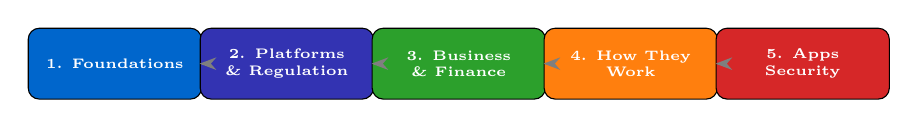
\begin{tikzpicture}[scale=0.78]
  \node[draw,fill=mlblue,text=white,rounded corners=4pt,
        minimum width=2.2cm,minimum height=0.9cm,align=center,font=\tiny\bfseries]
        (b1) at (0,0) {1. Foundations};
  \node[draw,fill=mlpurple,text=white,rounded corners=4pt,
        minimum width=2.2cm,minimum height=0.9cm,align=center,font=\tiny\bfseries]
        (b2) at (2.8,0) {2. Platforms\\\& Regulation};
  \node[draw,fill=mlgreen,text=white,rounded corners=4pt,
        minimum width=2.2cm,minimum height=0.9cm,align=center,font=\tiny\bfseries]
        (b3) at (5.6,0) {3. Business\\\& Finance};
  \node[draw,fill=mlorange,text=white,rounded corners=4pt,
        minimum width=2.2cm,minimum height=0.9cm,align=center,font=\tiny\bfseries]
        (b4) at (8.4,0) {4. How They\\Work};
  \node[draw,fill=mlred,text=white,rounded corners=4pt,
        minimum width=2.2cm,minimum height=0.9cm,align=center,font=\tiny\bfseries]
        (b5) at (11.2,0) {5. Apps\\Security};
  \draw[-{Stealth[length=6pt]},thick,mlgray] (b1.east) -- (b2.west);
  \draw[-{Stealth[length=6pt]},thick,mlgray] (b2.east) -- (b3.west);
  \draw[-{Stealth[length=6pt]},thick,mlgray] (b3.east) -- (b4.west);
  \draw[-{Stealth[length=6pt]},thick,mlgray] (b4.east) -- (b5.west);
\end{tikzpicture}
\vspace{3mm}

\column{0.45\textwidth}
\begin{block}{Learning Objectives}
\footnotesize
\begin{itemize}
  \item Define smart contracts and distinguish them from traditional contracts
  \item Trace the history from Nick Szabo to modern platforms
  \item Identify real-world business applications across industries
  \item Describe execution on blockchain platforms (EVM, gas, oracles)
  \item Evaluate security challenges and limitations
  \item Assess future potential and regulatory landscape
\end{itemize}
\end{block}
\vspace{1mm}
\begin{block}{No Prerequisites}
\footnotesize
\begin{itemize}
  \item This is a standalone introductory lecture
  \item No prior blockchain knowledge required
\end{itemize}
\end{block}
\end{columns}
\bottomnote{Duration: 90 minutes | 5 sections | \textasciitilde56 frames | No prerequisites required}
\end{frame}

% Frame 3: Learning Objectives
\begin{frame}{Learning Objectives}
By the end of this lecture, you will be able to:
\begin{enumerate}
\item \textbf{Define} smart contracts and distinguish them from traditional legal contracts
\item \textbf{Explain} the historical evolution from Nick Szabo's concept to modern platforms
\item \textbf{Identify} real-world business applications across industries (supply chain, insurance, finance)
\item \textbf{Describe} how smart contracts execute on blockchain platforms (EVM, gas, oracles)
\item \textbf{Evaluate} security challenges and limitations of smart contract technology
\item \textbf{Assess} the future potential and current regulatory landscape
\end{enumerate}
\bottomnote{Bloom's taxonomy levels: Remember $\rightarrow$ Understand $\rightarrow$ Apply $\rightarrow$ Analyze $\rightarrow$ Evaluate $\rightarrow$ Create}
\end{frame}

%% ============================================================
%% SECTION 1: SMART CONTRACT FOUNDATIONS
%% ============================================================
\section{Smart Contract Foundations}

% Frame 4: Section 1 Divider
\begin{frame}{}
\begin{beamercolorbox}[sep=12pt,center,rounded=true,shadow=true]{palette quaternary}
  {\Large\bfseries Section 1: What Are Smart Contracts?}\\[6pt]
  {\normalsize Understanding the concept, history, properties, and platforms of self-executing code}
\end{beamercolorbox}
\vspace{4mm}
\begin{columns}[T]
\column{0.5\textwidth}
\begin{block}{What You Will Learn}
\footnotesize
\begin{itemize}
  \item The vending machine analogy and core concept
  \item Historical evolution from 1994 to present
  \item Key properties: trustlessness, immutability, transparency
  \item Major smart contract platforms compared
  \item Legal status and regulatory landscape
  \item Current limitations and security challenges
\end{itemize}
\end{block}
\column{0.5\textwidth}
\begin{block}{Frames in This Section}
\footnotesize
\begin{itemize}
  \item Frame 5: The Vending Machine Analogy
  \item Frame 6: History -- From Szabo to Ethereum
  \item Frame 7: Defining Smart Contracts
  \item Frame 8: Smart Contracts vs Traditional Contracts
  \item Frame 9: How Smart Contracts Execute
  \item Frame 10: The Role of Blockchain
  \item Frame 11: Key Properties -- Trustlessness
  \item Frame 12: Immutability and Transparency
  \item Frame 13: Smart Contract Platforms Overview
  \item Frame 14: Ethereum -- The Pioneer Platform
  \item Frame 15: Beyond Ethereum
  \item Frame 16: Legal Status of Smart Contracts
  \item Frame 17: Regulatory Landscape
  \item Frame 18: Current Limitations
  \item Frame 19: The Oracle Problem
  \item Frame 20: Security Challenges Overview
\end{itemize}
\end{block}
\end{columns}
\bottomnote{Section 1 of 3 | Frames 4--20}
\end{frame}

% Frame 5: The Vending Machine Analogy
\begin{frame}{The Vending Machine Analogy}
\begin{columns}[T]
\column{0.48\textwidth}
\begin{block}{Nick Szabo's Insight (1994)}
\footnotesize
A \textbf{vending machine} is the simplest form of a smart contract:
\begin{enumerate}
  \item User inserts exact payment
  \item Machine verifies amount
  \item If sufficient $\rightarrow$ dispense product
  \item If insufficient $\rightarrow$ reject and refund
\end{enumerate}
No human intermediary. No trust required. The machine \emph{enforces} the agreement.
\end{block}

\column{0.52\textwidth}
\vspace{2mm}
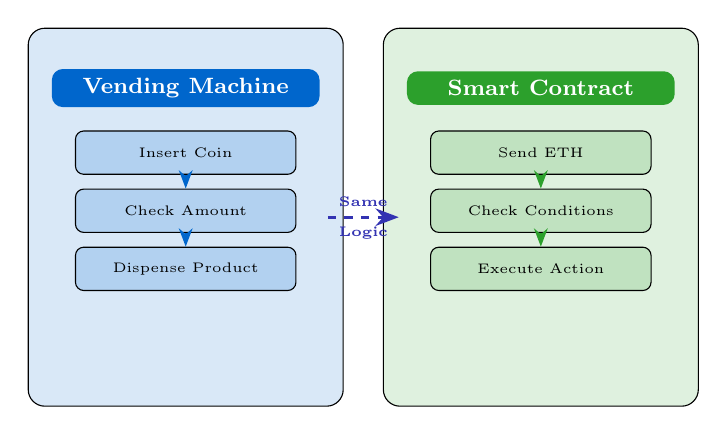
\begin{tikzpicture}[scale=0.82]
  % Vending Machine side
  \node[draw,fill=mlblue!15,rounded corners=6pt,
        minimum width=4.0cm,minimum height=4.8cm] at (0,0) {};
  \node[fill=mlblue,text=white,rounded corners=4pt,font=\footnotesize\bfseries,
        minimum width=3.4cm,align=center] at (0,2.0) {Vending Machine};
  \node[draw,fill=mlblue!30,rounded corners=3pt,font=\tiny,align=center,
        minimum width=2.8cm,minimum height=0.55cm] (v1) at (0,1.0) {Insert Coin};
  \node[draw,fill=mlblue!30,rounded corners=3pt,font=\tiny,align=center,
        minimum width=2.8cm,minimum height=0.55cm] (v2) at (0,0.1) {Check Amount};
  \node[draw,fill=mlblue!30,rounded corners=3pt,font=\tiny,align=center,
        minimum width=2.8cm,minimum height=0.55cm] (v3) at (0,-0.8) {Dispense Product};
  \draw[-{Stealth},thick,mlblue] (v1.south) -- (v2.north);
  \draw[-{Stealth},thick,mlblue] (v2.south) -- (v3.north);

  % Smart Contract side
  \node[draw,fill=mlgreen!15,rounded corners=6pt,
        minimum width=4.0cm,minimum height=4.8cm] at (5.5,0) {};
  \node[fill=mlgreen,text=white,rounded corners=4pt,font=\footnotesize\bfseries,
        minimum width=3.4cm,align=center] at (5.5,2.0) {Smart Contract};
  \node[draw,fill=mlgreen!30,rounded corners=3pt,font=\tiny,align=center,
        minimum width=2.8cm,minimum height=0.55cm] (s1) at (5.5,1.0) {Send ETH};
  \node[draw,fill=mlgreen!30,rounded corners=3pt,font=\tiny,align=center,
        minimum width=2.8cm,minimum height=0.55cm] (s2) at (5.5,0.1) {Check Conditions};
  \node[draw,fill=mlgreen!30,rounded corners=3pt,font=\tiny,align=center,
        minimum width=2.8cm,minimum height=0.55cm] (s3) at (5.5,-0.8) {Execute Action};
  \draw[-{Stealth},thick,mlgreen] (s1.south) -- (s2.north);
  \draw[-{Stealth},thick,mlgreen] (s2.south) -- (s3.north);

  % Connecting arrow
  \draw[-{Stealth},very thick,mlpurple,dashed] (2.2,0) -- (3.3,0)
        node[midway,above,font=\tiny\bfseries,text=mlpurple] {Same};
  \node[font=\tiny\bfseries,text=mlpurple] at (2.75,-0.25) {Logic};
\end{tikzpicture}
\end{columns}
\bottomnote{Nick Szabo coined ``smart contracts'' in 1994 -- the vending machine remains the best intuitive analogy for automated, trustless execution}
\end{frame}

% Frame 6: History: From Szabo to Ethereum
\begin{frame}{History: From Szabo to Ethereum}
\centering
\vspace{2mm}
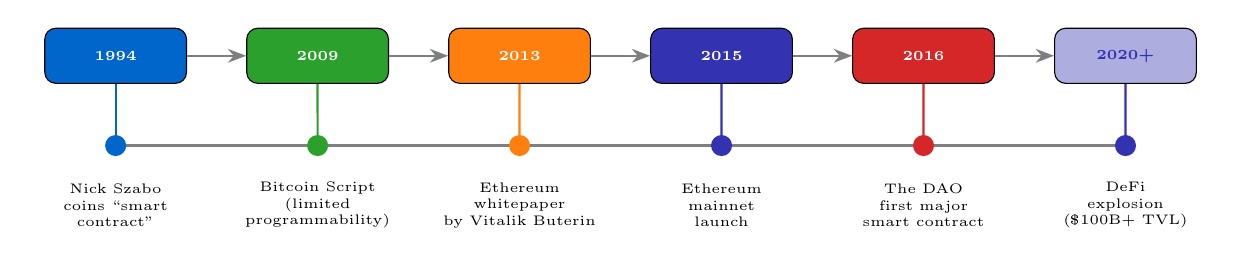
\begin{tikzpicture}[scale=0.95]
  % Timeline axis
  \draw[very thick,mlgray] (0,0) -- (13.5,0);

  % 1994
  \node[draw,fill=mlblue,text=white,rounded corners=4pt,
        minimum width=1.8cm,minimum height=0.7cm,align=center,font=\tiny\bfseries]
        (n1) at (0,1.2) {1994};
  \node[font=\tiny,align=center,text width=2.0cm] at (0,-0.8) {Nick Szabo\\coins ``smart\\contract''};
  \draw[thick,mlblue] (0,0.1) -- (n1.south);
  \fill[mlblue] (0,0) circle (4pt);

  % 2009
  \node[draw,fill=mlgreen,text=white,rounded corners=4pt,
        minimum width=1.8cm,minimum height=0.7cm,align=center,font=\tiny\bfseries]
        (n2) at (2.7,1.2) {2009};
  \node[font=\tiny,align=center,text width=2.0cm] at (2.7,-0.8) {Bitcoin Script\\(limited\\programmability)};
  \draw[thick,mlgreen] (2.7,0.1) -- (n2.south);
  \fill[mlgreen] (2.7,0) circle (4pt);

  % 2013
  \node[draw,fill=mlorange,text=white,rounded corners=4pt,
        minimum width=1.8cm,minimum height=0.7cm,align=center,font=\tiny\bfseries]
        (n3) at (5.4,1.2) {2013};
  \node[font=\tiny,align=center,text width=2.0cm] at (5.4,-0.8) {Ethereum\\whitepaper\\by Vitalik Buterin};
  \draw[thick,mlorange] (5.4,0.1) -- (n3.south);
  \fill[mlorange] (5.4,0) circle (4pt);

  % 2015
  \node[draw,fill=mlpurple,text=white,rounded corners=4pt,
        minimum width=1.8cm,minimum height=0.7cm,align=center,font=\tiny\bfseries]
        (n4) at (8.1,1.2) {2015};
  \node[font=\tiny,align=center,text width=2.0cm] at (8.1,-0.8) {Ethereum\\mainnet\\launch};
  \draw[thick,mlpurple] (8.1,0.1) -- (n4.south);
  \fill[mlpurple] (8.1,0) circle (4pt);

  % 2016
  \node[draw,fill=mlred,text=white,rounded corners=4pt,
        minimum width=1.8cm,minimum height=0.7cm,align=center,font=\tiny\bfseries]
        (n5) at (10.8,1.2) {2016};
  \node[font=\tiny,align=center,text width=2.0cm] at (10.8,-0.8) {The DAO\\first major\\smart contract};
  \draw[thick,mlred] (10.8,0.1) -- (n5.south);
  \fill[mlred] (10.8,0) circle (4pt);

  % 2020+
  \node[draw,fill=mllavender,text=mlpurple,rounded corners=4pt,
        minimum width=1.8cm,minimum height=0.7cm,align=center,font=\tiny\bfseries]
        (n6) at (13.5,1.2) {2020+};
  \node[font=\tiny,align=center,text width=2.0cm] at (13.5,-0.8) {DeFi\\explosion\\(\$100B+ TVL)};
  \draw[thick,mlpurple] (13.5,0.1) -- (n6.south);
  \fill[mlpurple] (13.5,0) circle (4pt);

  % Arrows between nodes
  \draw[-{Stealth},thick,mlgray] (n1.east) -- (n2.west);
  \draw[-{Stealth},thick,mlgray] (n2.east) -- (n3.west);
  \draw[-{Stealth},thick,mlgray] (n3.east) -- (n4.west);
  \draw[-{Stealth},thick,mlgray] (n4.east) -- (n5.west);
  \draw[-{Stealth},thick,mlgray] (n5.east) -- (n6.west);
\end{tikzpicture}
\vspace{3mm}
\begin{columns}[T]
\column{0.5\textwidth}
\begin{block}{Key Milestones}
\footnotesize
\begin{itemize}
  \item \textbf{1994}: Theoretical concept -- no blockchain existed
  \item \textbf{2009}: Bitcoin enabled limited scripting (e.g., multisig)
  \item \textbf{2013--2015}: Ethereum introduced Turing-complete smart contracts
\end{itemize}
\end{block}
\column{0.5\textwidth}
\begin{block}{The Turning Point}
\footnotesize
\begin{itemize}
  \item \textbf{2016}: The DAO raised \$150M and was hacked -- proving both the power and risk
  \item \textbf{2020+}: DeFi protocols like Uniswap, Aave, and Compound demonstrated real utility
\end{itemize}
\end{block}
\end{columns}
\bottomnote{It took 21 years from concept (1994) to practical realization (2015) -- smart contracts required blockchain infrastructure to become viable}
\end{frame}

% Frame 7: Defining Smart Contracts
\begin{frame}{Defining Smart Contracts}
\begin{block}{Formal Definition}
A \textbf{smart contract} is a self-executing program stored on a blockchain that automatically enforces the terms of an agreement when predetermined conditions are met, without requiring intermediaries.
\end{block}
\vspace{3mm}
\begin{columns}[T]
\column{0.5\textwidth}
\begin{block}{Key Properties}
\footnotesize
\begin{itemize}
  \item \textbf{Deterministic}: Same input $\rightarrow$ same output, always
  \item \textbf{Immutable}: Cannot be changed after deployment
  \item \textbf{Self-executing}: Runs automatically when conditions are met
  \item \textbf{Trustless}: No intermediary needed to enforce terms
  \item \textbf{Transparent}: Source code visible to all participants
\end{itemize}
\end{block}

\column{0.5\textwidth}
\begin{exampleblock}{In Practice}
\footnotesize
A smart contract is \emph{not} a legal contract by default. It is:
\begin{itemize}
  \item A \textbf{program} deployed to a blockchain address
  \item \textbf{Triggered} by transactions from users or other contracts
  \item \textbf{Executed} by every validator node identically
  \item \textbf{Permanent} -- the bytecode remains on-chain forever
  \item \textbf{Composable} -- contracts can call other contracts
\end{itemize}
\end{exampleblock}
\end{columns}
\vspace{2mm}
\centering
\textcolor{mlpurple}{\textbf{``A smart contract is neither smart nor a contract''}} -- it is deterministic code enforced by consensus.
\bottomnote{The term ``smart contract'' is widely considered a misnomer -- the code does not understand intent and has no legal standing by default}
\end{frame}

% Frame 8: Smart Contracts vs Traditional Contracts
\begin{frame}{Smart Contracts vs Traditional Contracts}
\centering
\vspace{-1mm}
\begin{adjustbox}{max width=\textwidth}
\begin{tabular}{>{\bfseries}l l l}
\toprule
\textbf{Feature} & \textbf{Traditional Contract} & \textbf{Smart Contract} \\
\midrule
\rowcolor{mllavender4}
Enforcement & Courts / Legal system & Code / Blockchain consensus \\
Speed & Days to months & Seconds to minutes \\
\rowcolor{mllavender4}
Cost & Legal fees, intermediaries & Gas fees only \\
Trust & Relies on institutions & Relies on code (``code is law'') \\
\rowcolor{mllavender4}
Modification & Amendments possible & Immutable (mostly) \\
Jurisdiction & National / Regional & Global / Borderless \\
\rowcolor{mllavender4}
Ambiguity & Language can be vague & Code is precise and deterministic \\
Dispute Resolution & Arbitration, litigation & On-chain logic (no appeals) \\
\rowcolor{mllavender4}
Parties & Identified, vetted & Pseudonymous (any address) \\
Execution & Manual compliance needed & Automatic, guaranteed \\
\bottomrule
\end{tabular}
\end{adjustbox}
\vspace{3mm}
\begin{columns}[T]
\column{0.5\textwidth}
\begin{alertblock}{Traditional Advantage}
\footnotesize
Flexibility: courts can interpret \emph{intent}, handle edge cases, and provide remedies not foreseen in the original terms.
\end{alertblock}
\column{0.5\textwidth}
\begin{exampleblock}{Smart Contract Advantage}
\footnotesize
Certainty: execution is guaranteed, transparent, and cannot be blocked by any single party or government.
\end{exampleblock}
\end{columns}
\bottomnote{Enforcement mechanism is the fundamental difference -- legal systems interpret intent; smart contracts execute code literally}
\end{frame}

% Frame 9: How Smart Contracts Execute
\begin{frame}{How Smart Contracts Execute}
\centering
\vspace{2mm}
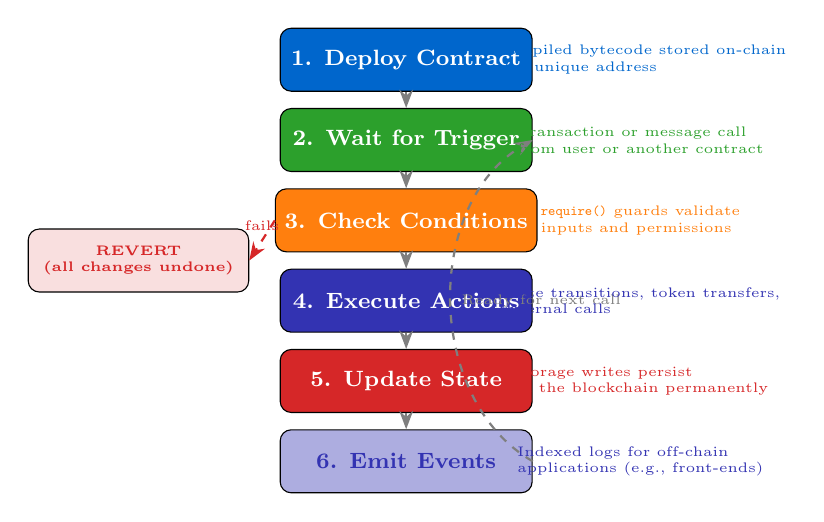
\begin{tikzpicture}[scale=0.85]
  % Nodes in vertical flow
  \node[draw,fill=mlblue,text=white,rounded corners=4pt,
        minimum width=3.2cm,minimum height=0.8cm,align=center,font=\footnotesize\bfseries]
        (n1) at (0,4.0) {1. Deploy Contract};
  \node[draw,fill=mlgreen,text=white,rounded corners=4pt,
        minimum width=3.2cm,minimum height=0.8cm,align=center,font=\footnotesize\bfseries]
        (n2) at (0,2.8) {2. Wait for Trigger};
  \node[draw,fill=mlorange,text=white,rounded corners=4pt,
        minimum width=3.2cm,minimum height=0.8cm,align=center,font=\footnotesize\bfseries]
        (n3) at (0,1.6) {3. Check Conditions};
  \node[draw,fill=mlpurple,text=white,rounded corners=4pt,
        minimum width=3.2cm,minimum height=0.8cm,align=center,font=\footnotesize\bfseries]
        (n4) at (0,0.4) {4. Execute Actions};
  \node[draw,fill=mlred,text=white,rounded corners=4pt,
        minimum width=3.2cm,minimum height=0.8cm,align=center,font=\footnotesize\bfseries]
        (n5) at (0,-0.8) {5. Update State};
  \node[draw,fill=mllavender,text=mlpurple,rounded corners=4pt,
        minimum width=3.2cm,minimum height=0.8cm,align=center,font=\footnotesize\bfseries]
        (n6) at (0,-2.0) {6. Emit Events};

  % Arrows
  \draw[-{Stealth},thick,mlgray] (n1.south) -- (n2.north);
  \draw[-{Stealth},thick,mlgray] (n2.south) -- (n3.north);
  \draw[-{Stealth},thick,mlgray] (n3.south) -- (n4.north);
  \draw[-{Stealth},thick,mlgray] (n4.south) -- (n5.north);
  \draw[-{Stealth},thick,mlgray] (n5.south) -- (n6.north);

  % Feedback loop
  \draw[-{Stealth},thick,mlgray,dashed] (n6.east) to[bend left=60] node[midway,right,font=\tiny,text=mlgray] {Ready for next call} (n2.east);

  % Annotations
  \node[font=\tiny,align=left,text=mlblue] at (3.5,4.0) {Compiled bytecode stored on-chain\\at a unique address};
  \node[font=\tiny,align=left,text=mlgreen] at (3.5,2.8) {Transaction or message call\\from user or another contract};
  \node[font=\tiny,align=left,text=mlorange] at (3.5,1.6) {\texttt{require()} guards validate\\inputs and permissions};
  \node[font=\tiny,align=left,text=mlpurple] at (3.5,0.4) {State transitions, token transfers,\\external calls};
  \node[font=\tiny,align=left,text=mlred] at (3.5,-0.8) {Storage writes persist\\on the blockchain permanently};
  \node[font=\tiny,align=left,text=mlpurple] at (3.5,-2.0) {Indexed logs for off-chain\\applications (e.g., front-ends)};

  % Revert box
  \node[draw,fill=mlred!15,rounded corners=4pt,
        minimum width=2.8cm,minimum height=0.8cm,align=center,font=\tiny\bfseries,text=mlred]
        (rev) at (-4.0,1.0) {REVERT\\(all changes undone)};
  \draw[-{Stealth},thick,mlred,dashed] (n3.west) -- (rev.east)
        node[midway,above,font=\tiny,text=mlred] {fails};
\end{tikzpicture}
\bottomnote{Smart contract execution is atomic -- if any step fails, the entire transaction reverts and gas is consumed but state remains unchanged}
\end{frame}

% Frame 10: The Role of Blockchain
\begin{frame}{The Role of Blockchain}
\begin{columns}[T]
\column{0.33\textwidth}
\begin{block}{\textcolor{mlblue}{Trust}}
\footnotesize
\begin{itemize}
  \item \textbf{Decentralized validation} -- thousands of nodes verify execution independently
  \item \textbf{No single point of failure} -- no server to hack or shut down
  \item \textbf{Consensus-enforced} -- majority must agree on state
  \item \textbf{Permissionless} -- anyone can deploy and interact
\end{itemize}
\end{block}

\column{0.33\textwidth}
\begin{block}{\textcolor{mlgreen}{Immutability}}
\footnotesize
\begin{itemize}
  \item \textbf{Once deployed}, code cannot be altered or deleted
  \item \textbf{Transaction history} is permanent and append-only
  \item \textbf{No rollbacks} (except hard forks -- extremely rare)
  \item \textbf{Cryptographic integrity} via hash chains
\end{itemize}
\end{block}

\column{0.33\textwidth}
\begin{block}{\textcolor{mlorange}{Transparency}}
\footnotesize
\begin{itemize}
  \item \textbf{Anyone can verify} contract logic on-chain
  \item \textbf{All transactions} are publicly auditable
  \item \textbf{Open source by default} -- bytecode always visible
  \item \textbf{Block explorers} (Etherscan) provide full visibility
\end{itemize}
\end{block}
\end{columns}
\vspace{4mm}
\centering
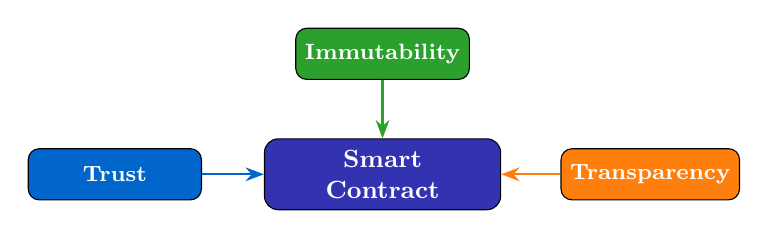
\begin{tikzpicture}[scale=0.85]
  \node[draw,fill=mlpurple,text=white,rounded corners=5pt,
        minimum width=3.0cm,minimum height=0.9cm,align=center,font=\small\bfseries]
        (sc) at (0,0) {Smart\\Contract};
  \node[draw,fill=mlblue,text=white,rounded corners=4pt,
        minimum width=2.2cm,minimum height=0.65cm,align=center,font=\footnotesize\bfseries]
        (t) at (-4.0,0) {Trust};
  \node[draw,fill=mlgreen,text=white,rounded corners=4pt,
        minimum width=2.2cm,minimum height=0.65cm,align=center,font=\footnotesize\bfseries]
        (i) at (0,1.8) {Immutability};
  \node[draw,fill=mlorange,text=white,rounded corners=4pt,
        minimum width=2.2cm,minimum height=0.65cm,align=center,font=\footnotesize\bfseries]
        (tr) at (4.0,0) {Transparency};
  \draw[-{Stealth},thick,mlblue] (t.east) -- (sc.west);
  \draw[-{Stealth},thick,mlgreen] (i.south) -- (sc.north);
  \draw[-{Stealth},thick,mlorange] (tr.west) -- (sc.east);
\end{tikzpicture}
\bottomnote{Blockchain provides the trust layer that makes smart contracts possible -- without it, self-executing code would need a trusted server}
\end{frame}

% Frame 11: Key Properties: Trustlessness
\begin{frame}{Key Properties: Trustlessness}
\begin{columns}[T]
\column{0.45\textwidth}
\begin{block}{``Code is Law''}
\footnotesize
The concept that \textbf{code replaces institutional trust}:
\begin{itemize}
  \item No bank, lawyer, or notary needed
  \item The contract itself is the neutral third party
  \item Execution is guaranteed by consensus
  \item Rules cannot be bent, reinterpreted, or ignored
  \item Both parties know the exact outcome in advance
\end{itemize}
\end{block}
\vspace{2mm}
\begin{alertblock}{Caveat}
\footnotesize
``Code is law'' only holds if the code is \emph{correct}. Bugs are enforced just as strictly as intended behavior.
\end{alertblock}

\column{0.55\textwidth}
\vspace{2mm}
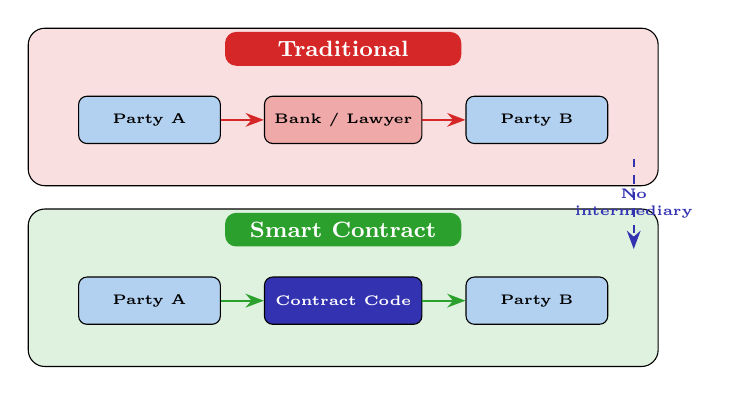
\begin{tikzpicture}[scale=0.82]
  % Traditional path
  \node[draw,fill=mlred!15,rounded corners=6pt,
        minimum width=8.0cm,minimum height=2.0cm] at (2.5,2.0) {};
  \node[fill=mlred,text=white,rounded corners=4pt,font=\footnotesize\bfseries,
        minimum width=3.0cm,align=center] at (2.5,2.9) {Traditional};
  \node[draw,fill=mlblue!30,rounded corners=3pt,font=\tiny\bfseries,align=center,
        minimum width=1.8cm,minimum height=0.6cm] (pa) at (-0.5,1.8) {Party A};
  \node[draw,fill=mlred!40,rounded corners=3pt,font=\tiny\bfseries,align=center,
        minimum width=2.0cm,minimum height=0.6cm] (mid) at (2.5,1.8) {Bank / Lawyer};
  \node[draw,fill=mlblue!30,rounded corners=3pt,font=\tiny\bfseries,align=center,
        minimum width=1.8cm,minimum height=0.6cm] (pb) at (5.5,1.8) {Party B};
  \draw[-{Stealth},thick,mlred] (pa.east) -- (mid.west);
  \draw[-{Stealth},thick,mlred] (mid.east) -- (pb.west);

  % Smart Contract path
  \node[draw,fill=mlgreen!15,rounded corners=6pt,
        minimum width=8.0cm,minimum height=2.0cm] at (2.5,-0.8) {};
  \node[fill=mlgreen,text=white,rounded corners=4pt,font=\footnotesize\bfseries,
        minimum width=3.0cm,align=center] at (2.5,0.1) {Smart Contract};
  \node[draw,fill=mlblue!30,rounded corners=3pt,font=\tiny\bfseries,align=center,
        minimum width=1.8cm,minimum height=0.6cm] (pa2) at (-0.5,-1.0) {Party A};
  \node[draw,fill=mlpurple,text=white,rounded corners=3pt,font=\tiny\bfseries,align=center,
        minimum width=2.0cm,minimum height=0.6cm] (sc2) at (2.5,-1.0) {Contract Code};
  \node[draw,fill=mlblue!30,rounded corners=3pt,font=\tiny\bfseries,align=center,
        minimum width=1.8cm,minimum height=0.6cm] (pb2) at (5.5,-1.0) {Party B};
  \draw[-{Stealth},thick,mlgreen] (pa2.east) -- (sc2.west);
  \draw[-{Stealth},thick,mlgreen] (sc2.east) -- (pb2.west);

  % Comparison label
  \node[font=\tiny\bfseries,text=mlpurple,align=center] at (7.0,0.5) {No\\intermediary};
  \draw[-{Stealth},thick,mlpurple,dashed] (7.0,1.2) -- (7.0,-0.2);
\end{tikzpicture}
\end{columns}
\bottomnote{Trust minimization is the core value proposition -- but shifts risk from institutions to code correctness}
\end{frame}

% Frame 12: Key Properties: Immutability and Transparency
\begin{frame}{Key Properties: Immutability and Transparency}
\begin{columns}[T]
\column{0.5\textwidth}
\begin{block}{\textcolor{mlblue}{Immutability}}
\footnotesize
Once a smart contract is deployed to the blockchain:
\begin{itemize}
  \item The \textbf{bytecode is permanent} -- it cannot be edited, patched, or deleted
  \item The \textbf{contract address} persists forever
  \item All \textbf{past transactions} remain in the history
  \item Even the \textbf{deployer} cannot modify the code
\end{itemize}
\end{block}
\vspace{2mm}
\begin{alertblock}{The Proxy Pattern (Caveat)}
\footnotesize
Developers use \textbf{proxy contracts} (EIP-1967) to achieve upgradeability:
\begin{itemize}
  \item Proxy stores state, delegates logic to implementation contract
  \item Implementation can be swapped $\rightarrow$ effectively ``mutable''
  \item Trade-off: upgradeability vs trust (who controls upgrades?)
\end{itemize}
\end{alertblock}

\column{0.5\textwidth}
\begin{block}{\textcolor{mlorange}{Transparency}}
\footnotesize
Smart contracts are open by design:
\begin{itemize}
  \item \textbf{Bytecode} is always visible on-chain
  \item \textbf{Verified source code} on Etherscan for most major projects
  \item \textbf{All transactions} are publicly auditable by anyone
  \item \textbf{State variables} can be read directly from the blockchain
  \item \textbf{Event logs} provide a searchable history of all actions
\end{itemize}
\end{block}
\vspace{2mm}
\begin{exampleblock}{Double-Edged Sword}
\footnotesize
Transparency means:
\begin{itemize}
  \item Anyone can audit for bugs (good for security)
  \item Attackers can also study the code (risk for exploits)
  \item No ``security through obscurity'' is possible
\end{itemize}
\end{exampleblock}
\end{columns}
\bottomnote{Immutability is a double-edged sword -- it guarantees contract integrity but makes bug fixes impossible without proxy patterns}
\end{frame}

%% ============================================================
%% SECTION 2: PLATFORMS AND REGULATORY LANDSCAPE
%% ============================================================
\section{Platforms and Regulatory Landscape}

% Frame 13: Smart Contract Platforms Overview
\begin{frame}{Smart Contract Platforms Overview}
\centering
\vspace{-1mm}
\begin{adjustbox}{max width=\textwidth}
\begin{tabular}{>{\bfseries}l c c c l}
\toprule
\textbf{Platform} & \textbf{Language} & \textbf{Consensus} & \textbf{TPS} & \textbf{Notable Feature} \\
\midrule
\rowcolor{mllavender4}
Ethereum & Solidity / Vyper & Proof of Stake & \textasciitilde30 & Largest ecosystem, EVM standard \\
Solana & Rust / C & PoH + PoS & \textasciitilde65,000 & High throughput, low latency \\
\rowcolor{mllavender4}
Cardano & Plutus / Haskell & Ouroboros PoS & \textasciitilde250 & Formal verification, eUTXO \\
Avalanche & Solidity (EVM) & Avalanche Consensus & \textasciitilde4,500 & Subnets, sub-second finality \\
\rowcolor{mllavender4}
Polkadot & ink! (Rust) & NPoS & \textasciitilde1,000 & Parachains, cross-chain \\
BNB Chain & Solidity (EVM) & PoSA & \textasciitilde160 & Low fees, CeFi integration \\
\rowcolor{mllavender4}
Tezos & Michelson & LPoS & \textasciitilde40 & On-chain governance, upgrades \\
\bottomrule
\end{tabular}
\end{adjustbox}
\vspace{3mm}
\begin{columns}[T]
\column{0.5\textwidth}
\begin{block}{EVM-Compatible Chains}
\footnotesize
\begin{itemize}
  \item Ethereum, Avalanche, BNB Chain, Polygon, Arbitrum share the \textbf{Ethereum Virtual Machine}
  \item Developers can deploy the \textbf{same Solidity code} across all EVM chains
  \item EVM is the de facto industry standard
\end{itemize}
\end{block}
\column{0.5\textwidth}
\begin{block}{Non-EVM Innovators}
\footnotesize
\begin{itemize}
  \item \textbf{Solana}: Parallel execution, Sealevel runtime
  \item \textbf{Cardano}: Academic rigor, peer-reviewed protocols
  \item \textbf{Polkadot}: Heterogeneous sharding via parachains
\end{itemize}
\end{block}
\end{columns}
\bottomnote{Ethereum dominates with \textasciitilde60\% of total smart contract TVL -- EVM compatibility is the most common strategy for new chains}
\end{frame}

% Frame 14: Ethereum: The Pioneer Platform
\begin{frame}{Ethereum: The Pioneer Platform}
\begin{columns}[T]
\column{0.5\textwidth}
\begin{block}{Ecosystem Dominance}
\footnotesize
\begin{itemize}
  \item \textbf{\textasciitilde4,000+ monthly active developers} -- largest Web3 dev community
  \item \textbf{\$40B+ TVL} locked in DeFi protocols
  \item \textbf{500,000+} deployed smart contracts
  \item \textbf{EVM} adopted by 20+ chains as the execution standard
  \item \textbf{Tooling}: Hardhat, Foundry, Remix, OpenZeppelin
\end{itemize}
\end{block}
\vspace{2mm}
\begin{block}{Post-Merge Ethereum (PoS)}
\footnotesize
\begin{itemize}
  \item Transitioned from Proof of Work to \textbf{Proof of Stake} (Sep 2022)
  \item \textbf{99.95\% energy reduction}
  \item \textbf{Staking yield} \textasciitilde3--5\% APR
  \item \textbf{Deflationary} via EIP-1559 base fee burn
\end{itemize}
\end{block}

\column{0.5\textwidth}
\begin{block}{ERC Token Standards}
\footnotesize
\begin{itemize}
  \item \textbf{ERC-20}: Fungible tokens (USDC, UNI, LINK)
  \item \textbf{ERC-721}: Non-fungible tokens (NFTs -- CryptoPunks, BAYC)
  \item \textbf{ERC-1155}: Multi-token standard (gaming, batch transfers)
  \item \textbf{ERC-4626}: Tokenized vaults (DeFi yield)
  \item \textbf{ERC-6551}: Token-bound accounts (NFTs owning assets)
\end{itemize}
\end{block}
\vspace{2mm}
\begin{exampleblock}{Layer 2 Scaling}
\footnotesize
\begin{itemize}
  \item \textbf{Arbitrum}: Optimistic rollup, \textasciitilde\$10B TVL
  \item \textbf{Optimism}: Optimistic rollup, OP Stack
  \item \textbf{zkSync}: ZK rollup, native account abstraction
  \item \textbf{Base}: Coinbase L2, onboarding focus
\end{itemize}
\end{exampleblock}
\end{columns}
\bottomnote{Ethereum's dominance is driven by network effects -- the largest developer community, deepest liquidity, and most battle-tested infrastructure}
\end{frame}

% Frame 15: Beyond Ethereum: Alternative Platforms
\begin{frame}{Beyond Ethereum: Alternative Platforms}
\begin{columns}[T]
\column{0.33\textwidth}
\begin{block}{\textcolor{mlblue}{Solana}}
\footnotesize
\begin{itemize}
  \item \textbf{Speed}: 400ms block time
  \item \textbf{Cost}: \textasciitilde\$0.00025 per transaction
  \item \textbf{Architecture}: Proof of History + PoS enables parallel transaction processing
  \item \textbf{Language}: Rust (systems-level control)
  \item \textbf{Ecosystem}: Jupiter, Marinade, Raydium
  \item \textbf{Trade-off}: Higher hardware requirements for validators
\end{itemize}
\end{block}

\column{0.33\textwidth}
\begin{block}{\textcolor{mlgreen}{Cardano}}
\footnotesize
\begin{itemize}
  \item \textbf{Approach}: Academic, peer-reviewed research
  \item \textbf{Formal verification}: Mathematically provable correctness
  \item \textbf{eUTXO model}: Extended UTXO for deterministic execution
  \item \textbf{Language}: Plutus (Haskell-based)
  \item \textbf{Governance}: On-chain voting (Project Catalyst)
  \item \textbf{Trade-off}: Slower development pace
\end{itemize}
\end{block}

\column{0.33\textwidth}
\begin{block}{\textcolor{mlorange}{Polkadot}}
\footnotesize
\begin{itemize}
  \item \textbf{Interoperability}: Heterogeneous multi-chain
  \item \textbf{Parachains}: Application-specific blockchains
  \item \textbf{Cross-chain}: Native message passing (XCM)
  \item \textbf{Language}: ink! (Rust-based, WASM)
  \item \textbf{Shared security}: Relay chain secures all parachains
  \item \textbf{Trade-off}: Complex parachain auction model
\end{itemize}
\end{block}
\end{columns}
\vspace{3mm}
\centering
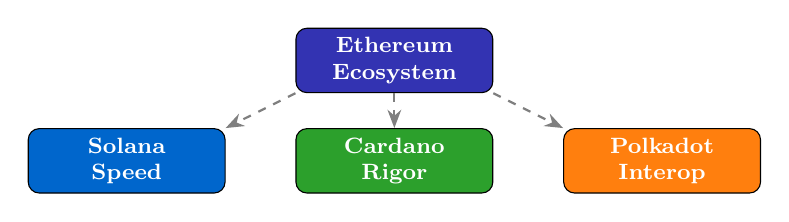
\begin{tikzpicture}[scale=0.85]
  \node[draw,fill=mlblue,text=white,rounded corners=4pt,
        minimum width=2.5cm,minimum height=0.7cm,align=center,font=\footnotesize\bfseries]
        (sol) at (0,0) {Solana\\Speed};
  \node[draw,fill=mlgreen,text=white,rounded corners=4pt,
        minimum width=2.5cm,minimum height=0.7cm,align=center,font=\footnotesize\bfseries]
        (car) at (4.0,0) {Cardano\\Rigor};
  \node[draw,fill=mlorange,text=white,rounded corners=4pt,
        minimum width=2.5cm,minimum height=0.7cm,align=center,font=\footnotesize\bfseries]
        (dot) at (8.0,0) {Polkadot\\Interop};
  \node[draw,fill=mlpurple,text=white,rounded corners=4pt,
        minimum width=2.5cm,minimum height=0.7cm,align=center,font=\footnotesize\bfseries]
        (eth) at (4.0,1.5) {Ethereum\\Ecosystem};
  \draw[-{Stealth},thick,mlgray,dashed] (eth.south west) -- (sol.north east);
  \draw[-{Stealth},thick,mlgray,dashed] (eth.south) -- (car.north);
  \draw[-{Stealth},thick,mlgray,dashed] (eth.south east) -- (dot.north west);
\end{tikzpicture}
\bottomnote{The future is likely multi-chain -- each platform optimizes for different trade-offs (speed, security, interoperability, formal correctness)}
\end{frame}

% Frame 16: Legal Status of Smart Contracts
\begin{frame}{Legal Status of Smart Contracts}
\begin{columns}[T]
\column{0.5\textwidth}
\begin{block}{Key Legal Questions}
\footnotesize
\begin{itemize}
  \item \textbf{Is code a contract?} -- Most jurisdictions say \emph{not automatically}
  \item \textbf{Offer and acceptance}: Can be expressed via transactions
  \item \textbf{Consideration}: ETH/tokens as payment may qualify
  \item \textbf{Intent}: Code does not capture subjective intent
  \item \textbf{Capacity}: Pseudonymous parties -- age/capacity unknown
\end{itemize}
\end{block}
\vspace{2mm}
\begin{block}{Ricardian Contracts}
\footnotesize
A \textbf{Ricardian contract} bridges the gap:
\begin{itemize}
  \item Legal prose (human-readable) \textbf{+} machine-readable code
  \item Both representations are cryptographically linked
  \item Legal terms govern intent; code governs execution
  \item Used by OpenLaw, Accord Project, Juro
\end{itemize}
\end{block}

\column{0.5\textwidth}
\begin{block}{Jurisdictions Recognizing Smart Contracts}
\footnotesize
\begin{itemize}
  \item \textbf{Wyoming, USA}: First state to legally recognize smart contracts (2019)
  \item \textbf{Tennessee, USA}: Smart contracts given legal effect under state law
  \item \textbf{Arizona, USA}: Smart contract signatures recognized
  \item \textbf{UK}: Law Commission recognizes crypto-assets and smart legal contracts
  \item \textbf{Singapore}: Smart contracts enforceable under existing contract law
\end{itemize}
\end{block}
\vspace{2mm}
\begin{exampleblock}{EU: MiCA Framework}
\footnotesize
The \textbf{Markets in Crypto-Assets} regulation (2024):
\begin{itemize}
  \item Licensing for crypto-asset service providers
  \item Stablecoin reserve requirements
  \item Does not directly regulate smart contract code
\end{itemize}
\end{exampleblock}
\end{columns}
\bottomnote{Legal uncertainty remains the biggest non-technical barrier -- most smart contracts operate in a legal gray area across jurisdictions}
\end{frame}

% Frame 17: Regulatory Landscape
\begin{frame}{Regulatory Landscape}
\begin{columns}[T]
\column{0.33\textwidth}
\begin{block}{\textcolor{mlblue}{United States}}
\footnotesize
\begin{itemize}
  \item \textbf{SEC}: Enforcement-driven approach; tokens as securities (Howey test)
  \item \textbf{CFTC}: Jurisdiction over crypto derivatives and commodities
  \item \textbf{State-level}: Wyoming, Tennessee, Arizona recognize smart contracts
  \item \textbf{IRS}: Crypto treated as property for tax purposes
  \item \textbf{FinCEN}: AML/KYC obligations for service providers
\end{itemize}
\end{block}

\column{0.33\textwidth}
\begin{block}{\textcolor{mlgreen}{European Union}}
\footnotesize
\begin{itemize}
  \item \textbf{MiCA}: Comprehensive crypto regulation (effective 2024)
  \item \textbf{Pilot Regime}: DLT sandbox for market infrastructure
  \item \textbf{DORA}: Digital operational resilience for financial entities
  \item \textbf{GDPR tension}: Right to deletion vs blockchain immutability
  \item \textbf{ECB}: Digital Euro CBDC exploration
\end{itemize}
\end{block}

\column{0.33\textwidth}
\begin{block}{\textcolor{mlorange}{Asia-Pacific}}
\footnotesize
\begin{itemize}
  \item \textbf{Singapore}: MAS regulatory sandbox; progressive framework
  \item \textbf{Japan}: FSA licensing regime; stablecoin regulation
  \item \textbf{Hong Kong}: New licensing for virtual asset providers
  \item \textbf{South Korea}: Virtual Asset User Protection Act
  \item \textbf{China}: Complete ban on crypto trading and mining
\end{itemize}
\end{block}
\end{columns}
\vspace{3mm}
\centering
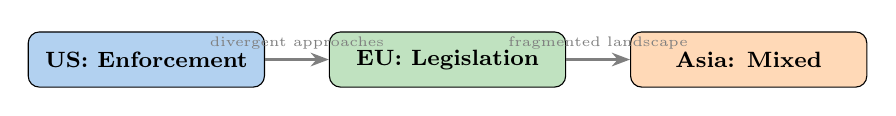
\begin{tikzpicture}[scale=0.85]
  \node[draw,fill=mlblue!30,rounded corners=4pt,
        minimum width=3.0cm,minimum height=0.7cm,align=center,font=\footnotesize\bfseries]
        (us) at (0,0) {US: Enforcement};
  \node[draw,fill=mlgreen!30,rounded corners=4pt,
        minimum width=3.0cm,minimum height=0.7cm,align=center,font=\footnotesize\bfseries]
        (eu) at (4.5,0) {EU: Legislation};
  \node[draw,fill=mlorange!30,rounded corners=4pt,
        minimum width=3.0cm,minimum height=0.7cm,align=center,font=\footnotesize\bfseries]
        (asia) at (9.0,0) {Asia: Mixed};
  \draw[-{Stealth},thick,mlgray] (us.east) -- (eu.west)
        node[midway,above,font=\tiny,text=mlgray] {divergent approaches};
  \draw[-{Stealth},thick,mlgray] (eu.east) -- (asia.west)
        node[midway,above,font=\tiny,text=mlgray] {fragmented landscape};
\end{tikzpicture}
\bottomnote{Regulation is evolving rapidly -- the EU's MiCA is the most comprehensive framework; the US relies primarily on enforcement actions}
\end{frame}

% Frame 18: Current Limitations
\begin{frame}{Current Limitations}
\begin{columns}[T]
\column{0.5\textwidth}
\begin{block}{Technical Limitations}
\footnotesize
\begin{itemize}
  \item \textbf{Scalability}: Limited throughput on most chains (Ethereum: \textasciitilde30 TPS vs Visa: \textasciitilde65,000 TPS)
  \item \textbf{Oracle Problem}: Cannot access off-chain data natively -- must rely on external data feeds
  \item \textbf{Immutability}: Bugs are permanent once deployed; no hotfixes possible
  \item \textbf{Gas Costs}: Can be expensive during network congestion (\$50--\$200+ per complex transaction)
  \item \textbf{Storage}: On-chain storage is extremely expensive (\textasciitilde\$16,000 per MB on Ethereum)
\end{itemize}
\end{block}

\column{0.5\textwidth}
\begin{block}{Non-Technical Limitations}
\footnotesize
\begin{itemize}
  \item \textbf{Legal Ambiguity}: Uncertain enforceability across jurisdictions
  \item \textbf{Complexity}: Hard to write bug-free code; Solidity has many footguns
  \item \textbf{User Experience}: Wallets, gas fees, and key management are confusing
  \item \textbf{Irreversibility}: No ``undo'' button; mistakes are permanent
  \item \textbf{Privacy}: All transactions and state are publicly visible
\end{itemize}
\end{block}
\end{columns}
\vspace{3mm}
\centering
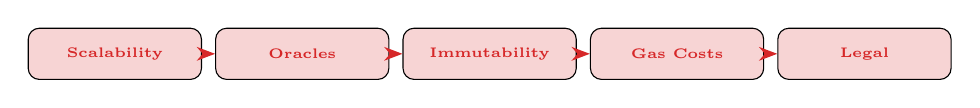
\begin{tikzpicture}[scale=0.85]
  \node[draw,fill=mlred!20,rounded corners=4pt,
        minimum width=2.2cm,minimum height=0.65cm,align=center,font=\tiny\bfseries,text=mlred]
        (l1) at (0,0) {Scalability};
  \node[draw,fill=mlred!20,rounded corners=4pt,
        minimum width=2.2cm,minimum height=0.65cm,align=center,font=\tiny\bfseries,text=mlred]
        (l2) at (2.8,0) {Oracles};
  \node[draw,fill=mlred!20,rounded corners=4pt,
        minimum width=2.2cm,minimum height=0.65cm,align=center,font=\tiny\bfseries,text=mlred]
        (l3) at (5.6,0) {Immutability};
  \node[draw,fill=mlred!20,rounded corners=4pt,
        minimum width=2.2cm,minimum height=0.65cm,align=center,font=\tiny\bfseries,text=mlred]
        (l4) at (8.4,0) {Gas Costs};
  \node[draw,fill=mlred!20,rounded corners=4pt,
        minimum width=2.2cm,minimum height=0.65cm,align=center,font=\tiny\bfseries,text=mlred]
        (l5) at (11.2,0) {Legal};
  \draw[-{Stealth},thick,mlred] (l1.east) -- (l2.west);
  \draw[-{Stealth},thick,mlred] (l2.east) -- (l3.west);
  \draw[-{Stealth},thick,mlred] (l3.east) -- (l4.west);
  \draw[-{Stealth},thick,mlred] (l4.east) -- (l5.west);
\end{tikzpicture}
\bottomnote{These limitations are being actively addressed -- L2 scaling, Chainlink oracles, proxy patterns, and account abstraction tackle the biggest pain points}
\end{frame}

% Frame 19: The Oracle Problem
\begin{frame}{The Oracle Problem}
\begin{columns}[T]
\column{0.45\textwidth}
\begin{block}{The Problem}
\footnotesize
Smart contracts are \textbf{sandboxed} -- they can only access data already on the blockchain. They \emph{cannot}:
\begin{itemize}
  \item Call external APIs or websites
  \item Read stock prices or weather data
  \item Verify real-world events
  \item Access randomness (deterministic execution)
\end{itemize}
\end{block}
\vspace{2mm}
\begin{block}{Oracle Solutions}
\footnotesize
\begin{itemize}
  \item \textbf{Chainlink}: Decentralized oracle network; 1,000+ data feeds; \$75B+ TVS (Total Value Secured)
  \item \textbf{Band Protocol}: Cross-chain oracle with IBC support
  \item \textbf{Pyth Network}: High-frequency financial data (Solana-native)
  \item \textbf{UMA}: Optimistic oracle with dispute resolution
  \item \textbf{API3}: First-party oracles (data providers run nodes)
\end{itemize}
\end{block}

\column{0.55\textwidth}
\vspace{2mm}
\centering
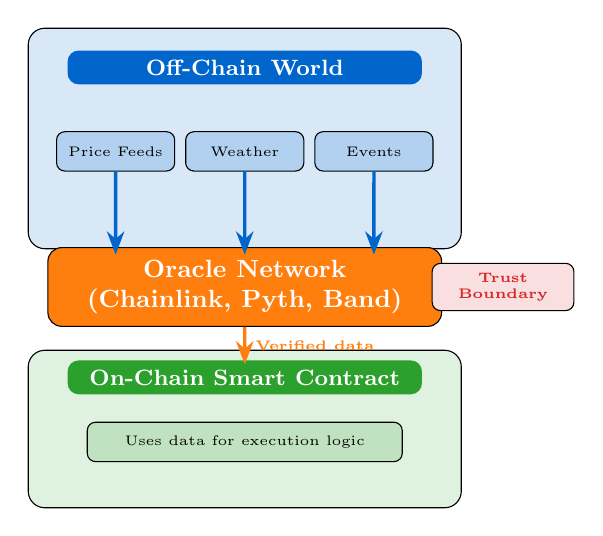
\begin{tikzpicture}[scale=0.82]
  % Off-chain world
  \node[draw,fill=mlblue!15,rounded corners=6pt,
        minimum width=5.5cm,minimum height=2.8cm] at (2.5,3.5) {};
  \node[fill=mlblue,text=white,rounded corners=4pt,font=\footnotesize\bfseries,
        minimum width=4.5cm,align=center] at (2.5,4.6) {Off-Chain World};
  \node[draw,fill=mlblue!30,rounded corners=3pt,font=\tiny,align=center,
        minimum width=1.5cm,minimum height=0.5cm] (d1) at (0.5,3.3) {Price Feeds};
  \node[draw,fill=mlblue!30,rounded corners=3pt,font=\tiny,align=center,
        minimum width=1.5cm,minimum height=0.5cm] (d2) at (2.5,3.3) {Weather};
  \node[draw,fill=mlblue!30,rounded corners=3pt,font=\tiny,align=center,
        minimum width=1.5cm,minimum height=0.5cm] (d3) at (4.5,3.3) {Events};

  % Oracle network
  \node[draw,fill=mlorange,text=white,rounded corners=5pt,
        minimum width=5.0cm,minimum height=1.0cm,align=center,font=\small\bfseries]
        (oracle) at (2.5,1.2) {Oracle Network\\(Chainlink, Pyth, Band)};

  % On-chain
  \node[draw,fill=mlgreen!15,rounded corners=6pt,
        minimum width=5.5cm,minimum height=2.0cm] at (2.5,-1.0) {};
  \node[fill=mlgreen,text=white,rounded corners=4pt,font=\footnotesize\bfseries,
        minimum width=4.5cm,align=center] at (2.5,-0.2) {On-Chain Smart Contract};
  \node[draw,fill=mlgreen!30,rounded corners=3pt,font=\tiny,align=center,
        minimum width=4.0cm,minimum height=0.5cm] (sc) at (2.5,-1.2) {Uses data for execution logic};

  % Arrows
  \draw[-{Stealth},very thick,mlblue] (d1.south) -- (0.5,1.7);
  \draw[-{Stealth},very thick,mlblue] (d2.south) -- (2.5,1.7);
  \draw[-{Stealth},very thick,mlblue] (d3.south) -- (4.5,1.7);
  \draw[-{Stealth},very thick,mlorange] (oracle.south) -- (2.5,-0.0)
        node[midway,right,font=\tiny\bfseries,text=mlorange] {Verified data};

  % Trust label
  \node[draw,fill=mlred!15,rounded corners=3pt,font=\tiny\bfseries,text=mlred,
        align=center,minimum width=1.8cm] at (6.5,1.2) {Trust\\Boundary};
\end{tikzpicture}
\end{columns}
\bottomnote{Chainlink is the dominant oracle solution, securing over \$75B in value -- the oracle is often the weakest link in smart contract security}
\end{frame}

% Frame 20: Security Challenges Overview
\begin{frame}{Security Challenges Overview}
\begin{columns}[T]
\column{0.5\textwidth}
\begin{block}{Why Security is Critical}
\footnotesize
\begin{itemize}
  \item \textbf{Bugs are permanent}: Once deployed, code cannot be patched (without proxies)
  \item \textbf{Financial incentive}: Contracts often hold millions in value, attracting attackers
  \item \textbf{Composability risk}: Contracts interact with other contracts, creating complex attack surfaces
  \item \textbf{Open source}: Attackers can study code at leisure before exploiting
  \item \textbf{Irreversibility}: Stolen funds cannot be recovered (no chargebacks)
\end{itemize}
\end{block}
\vspace{2mm}
\begin{block}{Smart Contract Auditing}
\footnotesize
\begin{itemize}
  \item Auditing is a \textbf{\$2B+ market} (growing 30\%+ annually)
  \item Top firms: Trail of Bits, OpenZeppelin, Consensys Diligence, Certora
  \item Typical audit: \$50K--\$500K for a complex protocol
  \item \textbf{Formal verification}: Mathematical proofs of correctness
  \item \textbf{Bug bounties}: Up to \$10M (Immunefi platform)
\end{itemize}
\end{block}

\column{0.5\textwidth}
\begin{alertblock}{Notable Smart Contract Failures}
\footnotesize
\begin{tabular}{l r l}
\toprule
\textbf{Incident} & \textbf{Loss} & \textbf{Year} \\
\midrule
\rowcolor{mllavender4}
The DAO & \$60M & 2016 \\
Parity Wallet & \$150M & 2017 \\
\rowcolor{mllavender4}
bZx Flash Loan & \$8M & 2020 \\
Wormhole Bridge & \$320M & 2022 \\
\rowcolor{mllavender4}
Ronin Bridge & \$625M & 2022 \\
Euler Finance & \$197M & 2023 \\
\bottomrule
\end{tabular}
\end{alertblock}
\vspace{2mm}
\begin{exampleblock}{Defense Layers}
\footnotesize
\begin{itemize}
  \item \textbf{Pre-deployment}: Audits, formal verification, test suites
  \item \textbf{Post-deployment}: Monitoring, circuit breakers, bug bounties
  \item \textbf{Design patterns}: Checks-effects-interactions, reentrancy guards, access control
\end{itemize}
\end{exampleblock}
\end{columns}
\bottomnote{Security is the top priority in smart contract development -- over \$3B has been lost to exploits; always audit before deploying to mainnet}
\end{frame}

%% ============================================================
%% SECTION 3: SMART CONTRACTS IN BUSINESS AND FINANCE
%% ============================================================
\section{Smart Contracts in Business and Finance}

% Frame 21: Section 2 Divider
\begin{frame}{}
\begin{beamercolorbox}[sep=12pt,center,rounded=true,shadow=true]{palette quaternary}
  {\Large\bfseries Section 2: Smart Contracts in Business \& Finance}\\[6pt]
  {\normalsize Why organizations care --- real-world applications across industries}
\end{beamercolorbox}
\vspace{4mm}
\begin{columns}[T]
\column{0.5\textwidth}
\begin{block}{What You Will Learn}
\footnotesize
\begin{itemize}
  \item Key business benefits: cost, speed, transparency
  \item Supply chain, insurance, and real estate applications
  \item Financial derivatives and trade finance automation
  \item DAOs as smart contract-governed organizations
  \item Healthcare, identity, and gaming use cases
  \item Enterprise adoption challenges and cost-benefit analysis
\end{itemize}
\end{block}
\column{0.5\textwidth}
\begin{block}{Frames in This Section}
\footnotesize
\begin{itemize}
  \item Frame 22: Why Businesses Care
  \item Frame 23: Supply Chain Management
  \item Frame 24: Supply Chain Case Study
  \item Frame 25: Parametric Insurance
  \item Frame 26: Insurance Case Study: Etherisc
  \item Frame 27: Real Estate and Property
  \item Frame 28: Financial Derivatives
  \item Frame 29: Trade Finance
  \item Frame 30: DAOs: Organizations as Code
  \item Frame 31: DAO Case Study: MakerDAO
  \item Frame 32: Healthcare Data Sharing
  \item Frame 33: Digital Identity
  \item Frame 34: Gaming and Digital Assets
  \item Frame 35: Enterprise Adoption Challenges
  \item Frame 36: Cost-Benefit Analysis
  \item Frame 37: The Disintermediation Thesis
\end{itemize}
\end{block}
\end{columns}
\bottomnote{Section 2 of 3 | Frames 21--37}
\end{frame}

% Frame 22: Why Businesses Care About Smart Contracts
\begin{frame}{Why Businesses Care About Smart Contracts}
\begin{columns}[T]
\column{0.25\textwidth}
\begin{block}{\textcolor{mlblue}{Cost Reduction}}
\footnotesize
\begin{itemize}
  \item Eliminate intermediaries (lawyers, brokers, notaries)
  \item Reduce administrative overhead
  \item Lower compliance costs
  \item No reconciliation needed
\end{itemize}
\end{block}

\column{0.25\textwidth}
\begin{block}{\textcolor{mlgreen}{Speed}}
\footnotesize
\begin{itemize}
  \item Settlement in seconds vs days
  \item 24/7 execution (no business hours)
  \item Instant finality on-chain
  \item No manual approval queues
\end{itemize}
\end{block}

\column{0.25\textwidth}
\begin{block}{\textcolor{mlorange}{Transparency}}
\footnotesize
\begin{itemize}
  \item All parties see the same data
  \item Auditable execution trail
  \item No hidden terms or side deals
  \item Real-time status tracking
\end{itemize}
\end{block}

\column{0.25\textwidth}
\begin{block}{\textcolor{mlpurple}{Disintermediation}}
\footnotesize
\begin{itemize}
  \item Direct peer-to-peer transactions
  \item No central authority needed
  \item Reduced counterparty risk
  \item Global access, borderless
\end{itemize}
\end{block}
\end{columns}
\vspace{4mm}
\centering
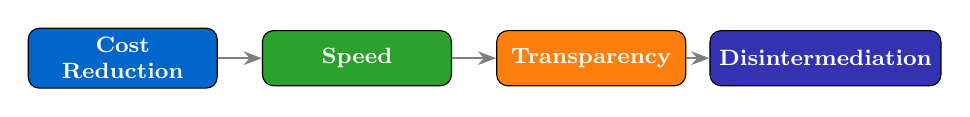
\begin{tikzpicture}[scale=0.85]
  \node[draw,fill=mlblue,text=white,rounded corners=4pt,
        minimum width=2.4cm,minimum height=0.7cm,align=center,font=\footnotesize\bfseries]
        (c1) at (0,0) {Cost\\Reduction};
  \node[draw,fill=mlgreen,text=white,rounded corners=4pt,
        minimum width=2.4cm,minimum height=0.7cm,align=center,font=\footnotesize\bfseries]
        (c2) at (3.5,0) {Speed};
  \node[draw,fill=mlorange,text=white,rounded corners=4pt,
        minimum width=2.4cm,minimum height=0.7cm,align=center,font=\footnotesize\bfseries]
        (c3) at (7.0,0) {Transparency};
  \node[draw,fill=mlpurple,text=white,rounded corners=4pt,
        minimum width=2.4cm,minimum height=0.7cm,align=center,font=\footnotesize\bfseries]
        (c4) at (10.5,0) {Disintermediation};
  \draw[-{Stealth},thick,mlgray] (c1.east) -- (c2.west);
  \draw[-{Stealth},thick,mlgray] (c2.east) -- (c3.west);
  \draw[-{Stealth},thick,mlgray] (c3.east) -- (c4.west);
\end{tikzpicture}
\bottomnote{The business value proposition is clear: smart contracts reduce costs by 50--95\%, accelerate settlement from days to seconds, and remove single points of failure}
\end{frame}

% Frame 23: Supply Chain Management
\begin{frame}{Supply Chain Management}
\begin{columns}[T]
\column{0.45\textwidth}
\begin{block}{How Smart Contracts Improve Supply Chains}
\footnotesize
\begin{itemize}
  \item \textbf{Provenance tracking}: Trace every product from source to consumer on an immutable ledger
  \item \textbf{Automated payments}: Release funds automatically upon delivery confirmation
  \item \textbf{Quality checkpoints}: IoT sensors trigger contract logic at each stage
  \item \textbf{Anti-counterfeiting}: Verify authenticity via on-chain certificates
  \item \textbf{Compliance}: Automated regulatory reporting at each node
\end{itemize}
\end{block}

\column{0.55\textwidth}
\vspace{2mm}
\centering
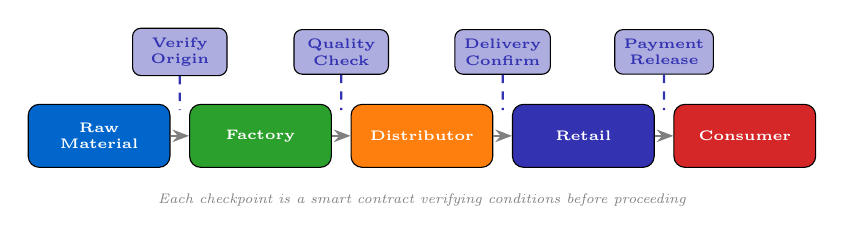
\begin{tikzpicture}[scale=0.82]
  % Supply chain nodes
  \node[draw,fill=mlblue,text=white,rounded corners=4pt,
        minimum width=1.8cm,minimum height=0.8cm,align=center,font=\tiny\bfseries]
        (r1) at (0,0) {Raw\\Material};
  \node[draw,fill=mlgreen,text=white,rounded corners=4pt,
        minimum width=1.8cm,minimum height=0.8cm,align=center,font=\tiny\bfseries]
        (r2) at (2.5,0) {Factory};
  \node[draw,fill=mlorange,text=white,rounded corners=4pt,
        minimum width=1.8cm,minimum height=0.8cm,align=center,font=\tiny\bfseries]
        (r3) at (5.0,0) {Distributor};
  \node[draw,fill=mlpurple,text=white,rounded corners=4pt,
        minimum width=1.8cm,minimum height=0.8cm,align=center,font=\tiny\bfseries]
        (r4) at (7.5,0) {Retail};
  \node[draw,fill=mlred,text=white,rounded corners=4pt,
        minimum width=1.8cm,minimum height=0.8cm,align=center,font=\tiny\bfseries]
        (r5) at (10.0,0) {Consumer};

  % Arrows between nodes
  \draw[-{Stealth[length=6pt]},thick,mlgray] (r1.east) -- (r2.west);
  \draw[-{Stealth[length=6pt]},thick,mlgray] (r2.east) -- (r3.west);
  \draw[-{Stealth[length=6pt]},thick,mlgray] (r3.east) -- (r4.west);
  \draw[-{Stealth[length=6pt]},thick,mlgray] (r4.east) -- (r5.west);

  % Smart contract checkpoints
  \node[draw,fill=mllavender,text=mlpurple,rounded corners=3pt,
        minimum width=1.2cm,minimum height=0.5cm,align=center,font=\tiny\bfseries]
        (sc1) at (1.25,1.3) {Verify\\Origin};
  \node[draw,fill=mllavender,text=mlpurple,rounded corners=3pt,
        minimum width=1.2cm,minimum height=0.5cm,align=center,font=\tiny\bfseries]
        (sc2) at (3.75,1.3) {Quality\\Check};
  \node[draw,fill=mllavender,text=mlpurple,rounded corners=3pt,
        minimum width=1.2cm,minimum height=0.5cm,align=center,font=\tiny\bfseries]
        (sc3) at (6.25,1.3) {Delivery\\Confirm};
  \node[draw,fill=mllavender,text=mlpurple,rounded corners=3pt,
        minimum width=1.2cm,minimum height=0.5cm,align=center,font=\tiny\bfseries]
        (sc4) at (8.75,1.3) {Payment\\Release};

  % Dashed lines from checkpoints to chain
  \draw[dashed,thick,mlpurple] (sc1.south) -- (1.25,0.4);
  \draw[dashed,thick,mlpurple] (sc2.south) -- (3.75,0.4);
  \draw[dashed,thick,mlpurple] (sc3.south) -- (6.25,0.4);
  \draw[dashed,thick,mlpurple] (sc4.south) -- (8.75,0.4);

  % Label
  \node[font=\tiny\itshape,text=mlgray] at (5.0,-1.0) {Each checkpoint is a smart contract verifying conditions before proceeding};
\end{tikzpicture}
\end{columns}
\bottomnote{Smart contracts transform supply chains from opaque, document-heavy processes into transparent, automated pipelines with verifiable provenance}
\end{frame}

% Frame 24: Supply Chain Case Study
\begin{frame}{Supply Chain Case Study: Walmart \& IBM Food Trust}
\begin{columns}[T]
\column{0.5\textwidth}
\begin{alertblock}{The Problem}
\footnotesize
\begin{itemize}
  \item Food safety tracing took \textbf{7 days} to trace a product back to its farm
  \item In foodborne illness outbreaks, every hour matters
  \item Paper-based records were incomplete and unreliable
  \item No way to isolate contaminated batches quickly
\end{itemize}
\end{alertblock}
\vspace{2mm}
\begin{exampleblock}{The Solution}
\footnotesize
\begin{itemize}
  \item Blockchain-based supply chain tracking via \textbf{IBM Food Trust} (Hyperledger Fabric)
  \item Every supplier uploads provenance data at each step
  \item Smart contracts validate transitions and flag anomalies
  \item Immutable audit trail from farm to shelf
\end{itemize}
\end{exampleblock}

\column{0.5\textwidth}
\begin{block}{Results}
\footnotesize
\begin{itemize}
  \item Tracing time reduced from \textbf{7 days} to \textbf{2.2 seconds}
  \item \textbf{500+} suppliers onboarded across multiple countries
  \item Reduced food waste through better expiry tracking
  \item Improved consumer safety and recall precision
  \item Other retailers (Carrefour, Nestl\'{e}) followed suit
\end{itemize}
\end{block}
\vspace{2mm}
\centering
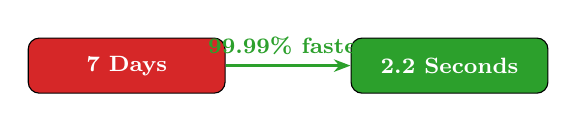
\begin{tikzpicture}[scale=0.82]
  \node[draw,fill=mlred,text=white,rounded corners=4pt,
        minimum width=2.5cm,minimum height=0.7cm,align=center,font=\footnotesize\bfseries]
        (old) at (0,0) {7 Days};
  \node[draw,fill=mlgreen,text=white,rounded corners=4pt,
        minimum width=2.5cm,minimum height=0.7cm,align=center,font=\footnotesize\bfseries]
        (new) at (5.0,0) {2.2 Seconds};
  \draw[-{Stealth[length=6pt]},very thick,mlgreen] (old.east) -- (new.west)
        node[midway,above,font=\footnotesize\bfseries,text=mlgreen] {99.99\% faster};
\end{tikzpicture}
\end{columns}
\bottomnote{Walmart's IBM Food Trust deployment is the most cited enterprise blockchain success story -- proving blockchain supply chain value at scale}
\end{frame}

% Frame 25: Insurance: Parametric Smart Contracts
\begin{frame}{Insurance: Parametric Smart Contracts}
\begin{columns}[T]
\column{0.45\textwidth}
\begin{block}{How Parametric Insurance Works}
\footnotesize
Parametric insurance replaces \emph{claims processes} with \emph{automatic triggers}:
\begin{itemize}
  \item \textbf{Weather-triggered payouts}: Rainfall exceeds threshold $\rightarrow$ automatic payment
  \item \textbf{Flight delay insurance}: Flight late $>$45 min $\rightarrow$ instant payout (no claim form)
  \item \textbf{Crop insurance}: Satellite data confirms drought $\rightarrow$ funds released
  \item \textbf{Natural disasters}: Seismic data triggers earthquake coverage
\end{itemize}
\vspace{2mm}
\textcolor{mlpurple}{\textbf{Key advantage:}} Remove human judgment from the claims process entirely.
\end{block}

\column{0.55\textwidth}
\vspace{2mm}
\centering
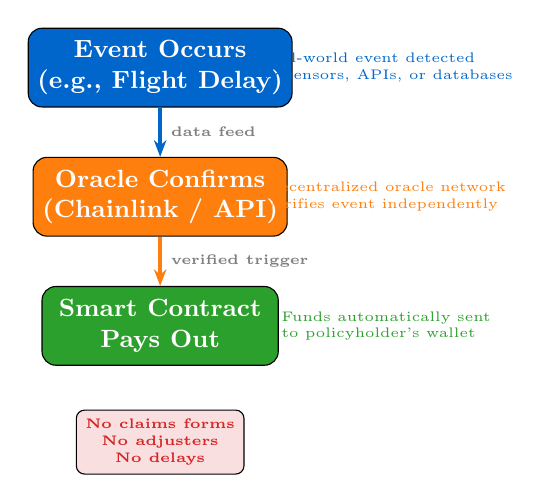
\begin{tikzpicture}[scale=0.82]
  % Event
  \node[draw,fill=mlblue,text=white,rounded corners=5pt,
        minimum width=3.0cm,minimum height=1.0cm,align=center,font=\small\bfseries]
        (ev) at (0,3.0) {Event Occurs\\(e.g., Flight Delay)};

  % Oracle
  \node[draw,fill=mlorange,text=white,rounded corners=5pt,
        minimum width=3.0cm,minimum height=1.0cm,align=center,font=\small\bfseries]
        (or) at (0,1.0) {Oracle Confirms\\(Chainlink / API)};

  % Smart Contract
  \node[draw,fill=mlgreen,text=white,rounded corners=5pt,
        minimum width=3.0cm,minimum height=1.0cm,align=center,font=\small\bfseries]
        (sc) at (0,-1.0) {Smart Contract\\Pays Out};

  % Arrows
  \draw[-{Stealth[length=6pt]},very thick,mlblue] (ev.south) -- (or.north)
        node[midway,right,font=\tiny\bfseries,text=mlgray] {data feed};
  \draw[-{Stealth[length=6pt]},very thick,mlorange] (or.south) -- (sc.north)
        node[midway,right,font=\tiny\bfseries,text=mlgray] {verified trigger};

  % Annotations
  \node[font=\tiny,align=left,text=mlblue] at (3.5,3.0) {Real-world event detected\\by sensors, APIs, or databases};
  \node[font=\tiny,align=left,text=mlorange] at (3.5,1.0) {Decentralized oracle network\\verifies event independently};
  \node[font=\tiny,align=left,text=mlgreen] at (3.5,-1.0) {Funds automatically sent\\to policyholder's wallet};

  % No claims box
  \node[draw,fill=mlred!15,rounded corners=3pt,font=\tiny\bfseries,text=mlred,
        align=center,minimum width=2.0cm] at (0,-2.8) {No claims forms\\No adjusters\\No delays};
\end{tikzpicture}
\end{columns}
\bottomnote{Parametric insurance eliminates the claims process entirely -- events trigger payouts automatically, reducing fraud and processing costs by over 90\%}
\end{frame}

% Frame 26: Insurance Case Study: Etherisc
\begin{frame}{Insurance Case Study: Etherisc}
\begin{columns}[T]
\column{0.5\textwidth}
\begin{block}{Etherisc Decentralized Insurance}
\footnotesize
\textbf{Etherisc} is a decentralized insurance protocol building parametric products on Ethereum:
\begin{itemize}
  \item Open-source insurance infrastructure
  \item Anyone can build insurance products on the platform
  \item Pooled risk across token holders
  \item Transparent claims handling via smart contracts
\end{itemize}
\end{block}
\vspace{2mm}
\begin{exampleblock}{Key Products}
\footnotesize
\begin{itemize}
  \item \textbf{Flight delay insurance}: Automatic payout if flight delayed $>$45 minutes; connected to FlightStats API via Chainlink
  \item \textbf{Crop insurance (Kenya)}: Satellite rainfall data triggers payouts to smallholder farmers
  \item \textbf{Hurricane protection}: Parametric triggers based on wind speed data
\end{itemize}
\end{exampleblock}

\column{0.5\textwidth}
\begin{block}{Impact and Adoption}
\footnotesize
\begin{tabular}{l l}
\toprule
\textbf{Metric} & \textbf{Value} \\
\midrule
\rowcolor{mllavender4}
Policies issued & 100,000+ \\
Farmer coverage (Kenya) & 17,000+ \\
\rowcolor{mllavender4}
Avg. payout time & Minutes \\
Traditional payout time & Weeks--months \\
\rowcolor{mllavender4}
Claims automation & 100\% \\
Admin cost reduction & $\sim$80\% \\
\bottomrule
\end{tabular}
\end{block}
\vspace{2mm}
\begin{alertblock}{Remaining Challenges}
\footnotesize
\begin{itemize}
  \item Oracle reliability is critical (garbage in $\rightarrow$ garbage out)
  \item Regulatory approval varies by jurisdiction
  \item Basis risk: parametric triggers may not match actual losses
\end{itemize}
\end{alertblock}
\end{columns}
\bottomnote{Etherisc demonstrates that decentralized insurance can serve underbanked populations -- Kenyan farmers receive payouts in minutes instead of months}
\end{frame}

% Frame 27: Real Estate and Property
\begin{frame}{Real Estate and Property}
\begin{columns}[T]
\column{0.5\textwidth}
\begin{block}{Smart Contracts in Real Estate}
\footnotesize
\begin{itemize}
  \item \textbf{Tokenized property}: Fractional ownership via ERC-20/ERC-1155 tokens -- invest in real estate with as little as \$50
  \item \textbf{Automated escrow}: Funds held in smart contract and released only when all conditions are met (inspection, title clear, signatures)
  \item \textbf{Title deed management}: On-chain property registry eliminates title fraud and duplicate claims
  \item \textbf{Rental agreements}: Automated rent collection, security deposit management, and maintenance escrow
\end{itemize}
\end{block}

\column{0.5\textwidth}
\begin{block}{Time and Cost Savings}
\footnotesize
\begin{tabular}{l l l}
\toprule
\textbf{Process} & \textbf{Traditional} & \textbf{Smart Contract} \\
\midrule
\rowcolor{mllavender4}
Closing time & 30--90 days & 1--3 days \\
Title search & \$500--\$1,500 & \$10--\$50 \\
\rowcolor{mllavender4}
Escrow fees & 1--2\% of price & $<$0.1\% \\
Agent commissions & 5--6\% & 1--2\% \\
\bottomrule
\end{tabular}
\end{block}
\vspace{2mm}
\begin{exampleblock}{Notable Projects}
\footnotesize
\begin{itemize}
  \item \textbf{RealT}: Tokenized US rental properties on Ethereum
  \item \textbf{Propy}: Completed first blockchain-recorded real estate sale (2017)
  \item \textbf{Lofty}: Tokenized property with daily rental income
\end{itemize}
\end{exampleblock}
\end{columns}
\bottomnote{Real estate tokenization could unlock \$280T in global property value -- making real estate as liquid and accessible as stocks}
\end{frame}

% Frame 28: Financial Derivatives and Settlements
\begin{frame}{Financial Derivatives and Settlements}
\begin{columns}[T]
\column{0.5\textwidth}
\begin{block}{Smart Contract-Based Finance}
\footnotesize
\begin{itemize}
  \item \textbf{Near-instant settlement}: Replaces T+2 (trade date + 2 days) with atomic settlement in a single transaction
  \item \textbf{Reduced counterparty risk}: Collateral locked in smart contracts, not held by intermediaries
  \item \textbf{Transparent margin management}: Real-time collateralization visible on-chain to all parties
  \item \textbf{Programmable derivatives}: Options, futures, and swaps encoded as smart contract logic
\end{itemize}
\end{block}
\vspace{2mm}
\begin{exampleblock}{DeFi Derivatives Protocols}
\footnotesize
\begin{itemize}
  \item \textbf{dYdX}: Decentralized perpetual futures (\$1B+ daily volume)
  \item \textbf{Synthetix}: Synthetic assets tracking real-world prices
  \item \textbf{GMX}: Decentralized spot and perpetual exchange
  \item \textbf{Opyn}: On-chain options protocol
\end{itemize}
\end{exampleblock}

\column{0.5\textwidth}
\vspace{2mm}
\centering
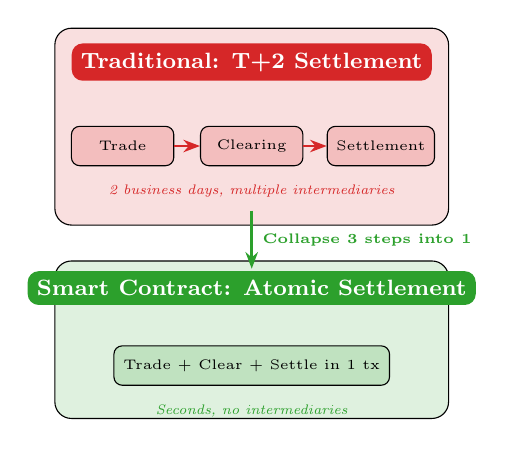
\begin{tikzpicture}[scale=0.82]
  % Traditional settlement
  \node[draw,fill=mlred!15,rounded corners=6pt,
        minimum width=5.0cm,minimum height=2.5cm] at (2.5,3.5) {};
  \node[fill=mlred,text=white,rounded corners=4pt,font=\footnotesize\bfseries,
        minimum width=4.5cm,align=center] at (2.5,4.5) {Traditional: T+2 Settlement};
  \node[draw,fill=mlred!30,rounded corners=3pt,font=\tiny,align=center,
        minimum width=1.3cm,minimum height=0.5cm] (t1) at (0.5,3.2) {Trade};
  \node[draw,fill=mlred!30,rounded corners=3pt,font=\tiny,align=center,
        minimum width=1.3cm,minimum height=0.5cm] (t2) at (2.5,3.2) {Clearing};
  \node[draw,fill=mlred!30,rounded corners=3pt,font=\tiny,align=center,
        minimum width=1.3cm,minimum height=0.5cm] (t3) at (4.5,3.2) {Settlement};
  \draw[-{Stealth[length=6pt]},thick,mlred] (t1.east) -- (t2.west);
  \draw[-{Stealth[length=6pt]},thick,mlred] (t2.east) -- (t3.west);
  \node[font=\tiny\itshape,text=mlred] at (2.5,2.5) {2 business days, multiple intermediaries};

  % Smart contract settlement
  \node[draw,fill=mlgreen!15,rounded corners=6pt,
        minimum width=5.0cm,minimum height=2.0cm] at (2.5,0.2) {};
  \node[fill=mlgreen,text=white,rounded corners=4pt,font=\footnotesize\bfseries,
        minimum width=4.5cm,align=center] at (2.5,1.0) {Smart Contract: Atomic Settlement};
  \node[draw,fill=mlgreen!30,rounded corners=3pt,font=\tiny,align=center,
        minimum width=3.5cm,minimum height=0.5cm] at (2.5,-0.2) {Trade + Clear + Settle in 1 tx};
  \node[font=\tiny\itshape,text=mlgreen] at (2.5,-0.9) {Seconds, no intermediaries};

  % Arrow between
  \draw[-{Stealth[length=6pt]},very thick,mlgreen] (2.5,2.2) -- (2.5,1.3)
        node[midway,right,font=\tiny\bfseries,text=mlgreen] {Collapse 3 steps into 1};
\end{tikzpicture}
\end{columns}
\bottomnote{The global derivatives market (\$700T+ notional) stands to benefit enormously from smart contract settlement -- reducing systemic risk and capital requirements}
\end{frame}

% Frame 29: Trade Finance and Letters of Credit
\begin{frame}{Trade Finance and Letters of Credit}
\begin{columns}[T]
\column{0.5\textwidth}
\begin{block}{The Trade Finance Problem}
\footnotesize
\begin{itemize}
  \item Cross-border trade involves \textbf{20+ documents} and \textbf{5--10 intermediaries}
  \item Letters of credit (LC) take \textbf{5--10 days} to process
  \item Paper-based documentation prone to fraud and errors
  \item \$1.7T trade finance gap (unmet demand, mostly in developing countries)
\end{itemize}
\end{block}
\vspace{2mm}
\begin{block}{Smart Contract Solutions}
\footnotesize
\begin{itemize}
  \item \textbf{Digital letters of credit}: Automated document verification and payment release
  \item \textbf{Cross-border payments}: Settlement in minutes instead of days
  \item \textbf{Document digitization}: Bills of lading, invoices, and certificates on-chain
  \item \textbf{Automated compliance}: KYC/AML checks embedded in contract logic
\end{itemize}
\end{block}

\column{0.5\textwidth}
\begin{exampleblock}{Enterprise Pilots}
\footnotesize
\begin{itemize}
  \item \textbf{HSBC}: Completed first blockchain-based letter of credit (2018); reduced processing from 5--10 days to 24 hours
  \item \textbf{Standard Chartered}: Trade finance on Ethereum for cross-border transactions
  \item \textbf{Contour}: Blockchain network for digital trade finance (70+ banks)
  \item \textbf{Marco Polo}: R3 Corda-based trade finance network
  \item \textbf{we.trade}: IBM-backed platform for European SME trade
\end{itemize}
\end{exampleblock}
\vspace{2mm}
\begin{alertblock}{Impact}
\footnotesize
Smart contract-based trade finance could close the \textbf{\$1.7T trade finance gap} by making financing accessible to SMEs in developing economies.
\end{alertblock}
\end{columns}
\bottomnote{Trade finance is one of the most promising enterprise blockchain use cases -- HSBC's LC pilot proved 80\% time reduction in real cross-border trade}
\end{frame}

% Frame 30: DAOs: Organizations as Smart Contracts
\begin{frame}{DAOs: Organizations as Smart Contracts}
\begin{columns}[T]
\column{0.5\textwidth}
\begin{block}{What is a DAO?}
\footnotesize
A \textbf{Decentralized Autonomous Organization} (DAO) is an organization governed entirely by smart contract rules rather than hierarchical management:
\begin{itemize}
  \item \textbf{Governance via code}: Proposals, voting, and execution happen on-chain
  \item \textbf{Token-based voting}: Governance tokens (e.g., UNI, AAVE) grant voting rights
  \item \textbf{Treasury management}: Funds held in smart contracts, released only by vote
  \item \textbf{Transparent operations}: Every decision and transaction is publicly auditable
\end{itemize}
\end{block}

\column{0.5\textwidth}
\begin{block}{Major DAOs}
\footnotesize
\begin{tabular}{l l l}
\toprule
\textbf{DAO} & \textbf{Purpose} & \textbf{Treasury} \\
\midrule
\rowcolor{mllavender4}
Uniswap & DEX governance & \$3B+ \\
MakerDAO & Stablecoin & \$8B+ TVL \\
\rowcolor{mllavender4}
Aave & Lending & \$10B+ TVL \\
Lido & Staking & \$15B+ TVL \\
\rowcolor{mllavender4}
Arbitrum & Layer 2 & \$3B+ \\
ENS & Name service & \$1B+ \\
\bottomrule
\end{tabular}
\end{block}
\vspace{2mm}
\begin{exampleblock}{Key Insight}
\footnotesize
DAOs represent a new organizational primitive -- \textbf{code replaces corporate bylaws}, and token holders replace shareholders.
\end{exampleblock}
\end{columns}
\bottomnote{DAOs are covered in depth in L09 -- here we focus on smart contracts as the enabling technology for decentralized governance}
\end{frame}

% Frame 31: DAO Case Study: MakerDAO
\begin{frame}{DAO Case Study: MakerDAO}
\begin{columns}[T]
\column{0.5\textwidth}
\begin{block}{Overview}
\footnotesize
\textbf{MakerDAO} is the largest decentralized lending protocol, governing the \textbf{DAI stablecoin} (pegged to \$1 USD):
\begin{itemize}
  \item Users lock collateral (ETH, WBTC, etc.) in smart contract ``vaults''
  \item Borrow DAI against collateral at algorithmically set interest rates
  \item Smart contracts automatically liquidate undercollateralized positions
  \item No bank, no credit check, no intermediary
\end{itemize}
\end{block}
\vspace{2mm}
\begin{block}{Governance}
\footnotesize
\begin{itemize}
  \item \textbf{MKR token} holders vote on risk parameters (collateral ratios, stability fees)
  \item Governance proposals go through on-chain voting
  \item Executive votes directly modify smart contract parameters
  \item \textbf{SubDAO structure} introduced for scalability (Spark, Sakura)
\end{itemize}
\end{block}

\column{0.5\textwidth}
\begin{block}{Key Statistics}
\footnotesize
\begin{tabular}{l l}
\toprule
\textbf{Metric} & \textbf{Value} \\
\midrule
\rowcolor{mllavender4}
Total Value Locked & \$8B+ \\
DAI in circulation & \$5B+ \\
\rowcolor{mllavender4}
Collateral types & 20+ \\
Active vaults & 50,000+ \\
\rowcolor{mllavender4}
Governance votes & 1,000+ \\
Revenue (annual) & \$150M+ \\
\bottomrule
\end{tabular}
\end{block}
\vspace{2mm}
\begin{alertblock}{Lessons Learned}
\footnotesize
\begin{itemize}
  \item Black Thursday (March 2020): \$8M in bad debt during market crash exposed liquidation system weaknesses
  \item Led to improved auction mechanisms and emergency shutdown procedures
  \item Voter apathy: $<$5\% of MKR holders vote regularly
\end{itemize}
\end{alertblock}
\end{columns}
\bottomnote{MakerDAO demonstrates both the power and complexity of DAO governance -- managing \$8B+ in TVL with decentralized decision-making}
\end{frame}

% Frame 32: Healthcare: Data Sharing and Consent
\begin{frame}{Healthcare: Data Sharing and Consent}
\begin{columns}[T]
\column{0.5\textwidth}
\begin{block}{Patient-Controlled Data Access}
\footnotesize
Smart contracts enable patients to control who accesses their health data:
\begin{itemize}
  \item \textbf{Granular permissions}: Grant/revoke access per provider, per data type, with time limits
  \item \textbf{Consent management}: On-chain consent records -- immutable proof of permission
  \item \textbf{Audit trails}: Every data access is logged transparently
  \item \textbf{Interoperability}: Cross-hospital data sharing without centralized databases
\end{itemize}
\end{block}
\vspace{2mm}
\begin{exampleblock}{Notable Projects}
\footnotesize
\begin{itemize}
  \item \textbf{MedRec} (MIT): Blockchain-based medical records
  \item \textbf{Solve.Care}: Healthcare administration platform
  \item \textbf{BurstIQ}: Health data marketplace with smart contracts
\end{itemize}
\end{exampleblock}

\column{0.5\textwidth}
\begin{block}{Clinical Trials}
\footnotesize
\begin{itemize}
  \item \textbf{Data integrity}: Trial results recorded on-chain -- cannot be altered retroactively
  \item \textbf{Consent tracking}: Patient consent stored immutably with timestamps
  \item \textbf{Automated payments}: Participants compensated automatically at milestones
  \item \textbf{Transparency}: Reduce publication bias by making all trial data verifiable
\end{itemize}
\end{block}
\vspace{2mm}
\begin{alertblock}{Privacy Considerations}
\footnotesize
\begin{itemize}
  \item Health data must \textbf{never} be stored directly on-chain (HIPAA/GDPR compliance)
  \item Only \textbf{access hashes} and \textbf{consent records} go on-chain
  \item Actual data remains in encrypted off-chain storage
  \item Zero-knowledge proofs can verify eligibility without revealing data
\end{itemize}
\end{alertblock}
\end{columns}
\bottomnote{Healthcare smart contracts manage access rights, not data itself -- the blockchain stores consent and audit trails while actual records remain in secure off-chain systems}
\end{frame}

% Frame 33: Digital Identity and Credentials
\begin{frame}{Digital Identity and Credentials}
\begin{columns}[T]
\column{0.5\textwidth}
\begin{block}{Self-Sovereign Identity (SSI)}
\footnotesize
\begin{itemize}
  \item \textbf{User-owned identity}: You control your digital identity, not platforms or governments
  \item \textbf{Portable credentials}: Use the same identity across services without re-verification
  \item \textbf{Selective disclosure}: Prove you are over 18 without revealing your birth date
  \item \textbf{No central database}: No honeypot for hackers to target
\end{itemize}
\end{block}
\vspace{2mm}
\begin{block}{KYC/AML Automation}
\footnotesize
\begin{itemize}
  \item Complete KYC once, reuse across platforms via verifiable credentials
  \item Smart contracts enforce AML rules automatically at transaction level
  \item Reduces compliance costs from \$500--\$5,000 per customer to near-zero for repeat verification
\end{itemize}
\end{block}

\column{0.5\textwidth}
\begin{block}{Verifiable Credentials}
\footnotesize
\begin{itemize}
  \item \textbf{Educational}: Universities issue diplomas as on-chain credentials (MIT, University of Bahrain)
  \item \textbf{Professional}: Licenses and certifications with automatic expiry tracking
  \item \textbf{Government}: Digital driver's licenses and national IDs
  \item \textbf{Employment}: Work history verified without contacting previous employers
\end{itemize}
\end{block}
\vspace{2mm}
\begin{exampleblock}{Standards and Projects}
\footnotesize
\begin{itemize}
  \item \textbf{W3C DID}: Decentralized Identifier standard
  \item \textbf{ENS}: Ethereum Name Service (human-readable addresses)
  \item \textbf{Worldcoin}: Proof of personhood via iris scans
  \item \textbf{Polygon ID}: Zero-knowledge identity framework
\end{itemize}
\end{exampleblock}
\end{columns}
\bottomnote{Self-sovereign identity shifts power from institutions to individuals -- you prove claims about yourself without surrendering your personal data}
\end{frame}

% Frame 34: Gaming and Digital Assets
\begin{frame}{Gaming and Digital Assets}
\begin{columns}[T]
\column{0.5\textwidth}
\begin{block}{True Digital Ownership}
\footnotesize
Smart contracts enable real ownership of in-game assets:
\begin{itemize}
  \item \textbf{NFT-based items}: Weapons, skins, and characters as tradeable tokens
  \item \textbf{Cross-game portability}: Use assets across different games and platforms
  \item \textbf{Player-owned economies}: In-game marketplaces governed by smart contracts
  \item \textbf{Verifiable scarcity}: Provably limited edition items (no duplication possible)
\end{itemize}
\end{block}
\vspace{2mm}
\begin{block}{Provably Fair Mechanics}
\footnotesize
\begin{itemize}
  \item Random number generation via Chainlink VRF (Verifiable Random Function)
  \item Game rules encoded in smart contracts -- no hidden manipulation
  \item Tournament prize pools held in escrow and distributed automatically
\end{itemize}
\end{block}

\column{0.5\textwidth}
\begin{block}{Notable Gaming Projects}
\footnotesize
\begin{tabular}{l l}
\toprule
\textbf{Project} & \textbf{Innovation} \\
\midrule
\rowcolor{mllavender4}
Axie Infinity & Play-to-earn pioneer \\
Illuvium & AAA-quality on-chain RPG \\
\rowcolor{mllavender4}
Gods Unchained & TCG with true ownership \\
The Sandbox & Virtual world + UGC \\
\rowcolor{mllavender4}
Immutable X & L2 for gas-free gaming \\
Ronin & Axie's dedicated sidechain \\
\bottomrule
\end{tabular}
\end{block}
\vspace{2mm}
\begin{alertblock}{Challenges}
\footnotesize
\begin{itemize}
  \item Play-to-earn sustainability (Axie economy collapsed)
  \item Onboarding friction (wallets, gas fees)
  \item Game quality often sacrificed for token mechanics
\end{itemize}
\end{alertblock}
\end{columns}
\bottomnote{Blockchain gaming's future lies in ownership and interoperability -- but game quality must come first; tokenomics alone cannot sustain player engagement}
\end{frame}

% Frame 35: Enterprise Adoption Challenges
\begin{frame}{Enterprise Adoption Challenges}
\begin{columns}[T]
\column{0.5\textwidth}
\begin{block}{Technical Barriers}
\footnotesize
\begin{itemize}
  \item \textbf{Legacy integration}: Most enterprises run SAP, Oracle, or custom systems that do not natively connect to blockchains
  \item \textbf{Scalability}: Public blockchains cannot handle enterprise transaction volumes (thousands of TPS needed)
  \item \textbf{Privacy}: Public chains expose all transaction data -- unacceptable for competitive business data
  \item \textbf{Interoperability}: No standard for cross-chain communication between enterprise networks
\end{itemize}
\end{block}
\vspace{2mm}
\begin{alertblock}{Talent Shortage}
\footnotesize
\begin{itemize}
  \item Only $\sim$30,000 active Solidity developers globally
  \item Demand exceeds supply by 5--10x
  \item Average Solidity developer salary: \$150K--\$250K
\end{itemize}
\end{alertblock}

\column{0.5\textwidth}
\begin{block}{Organizational Barriers}
\footnotesize
\begin{itemize}
  \item \textbf{Regulatory uncertainty}: Unclear compliance requirements create legal risk for adoption
  \item \textbf{Governance questions}: Who controls upgrades and bug fixes in a consortium?
  \item \textbf{Change management}: Employees resist processes that threaten their roles
  \item \textbf{ROI uncertainty}: Hard to quantify benefits before full deployment
\end{itemize}
\end{block}
\vspace{2mm}
\begin{exampleblock}{Private vs Public Chains}
\footnotesize
\begin{itemize}
  \item \textbf{Hyperledger Fabric}: Permissioned, private -- preferred by enterprises (IBM, Walmart)
  \item \textbf{R3 Corda}: Purpose-built for financial institutions
  \item \textbf{Public L2s}: Growing enterprise interest (Arbitrum, Polygon)
  \item Trade-off: privacy vs decentralization vs network effects
\end{itemize}
\end{exampleblock}
\end{columns}
\bottomnote{Enterprise adoption requires solving the trilemma of privacy, scalability, and decentralization -- private chains sacrifice decentralization; public chains sacrifice privacy}
\end{frame}

% Frame 36: Cost-Benefit Analysis
\begin{frame}{Cost-Benefit Analysis}
\centering
\vspace{-1mm}
\begin{adjustbox}{max width=\textwidth}
\begin{tabular}{>{\bfseries}l r r r}
\toprule
\textbf{Process} & \textbf{Traditional Cost} & \textbf{Smart Contract Cost} & \textbf{Savings} \\
\midrule
\rowcolor{mllavender4}
Cross-border payment & \$25--50 + 3--5 days & \$0.50 + seconds & 95\%+ \\
Insurance claim & \$500--2,000 + weeks & \$5--10 + minutes & 90\%+ \\
\rowcolor{mllavender4}
Property transfer & \$5,000--15,000 + months & \$50--200 + days & 95\%+ \\
Supply chain audit & \$10,000+ + weeks & \$100--500 + hours & 95\%+ \\
\rowcolor{mllavender4}
KYC verification & \$500--5,000 per customer & \$1--10 (reusable) & 99\%+ \\
Trade finance (LC) & \$5,000--50,000 + 5--10 days & \$100--500 + hours & 95\%+ \\
\rowcolor{mllavender4}
Derivatives settlement & Billions in capital + T+2 & Near-zero + seconds & 90\%+ \\
Contract notarization & \$200--500 per document & \$1--5 per hash & 98\%+ \\
\bottomrule
\end{tabular}
\end{adjustbox}
\vspace{4mm}
\begin{columns}[T]
\column{0.5\textwidth}
\begin{exampleblock}{Where Savings Are Greatest}
\footnotesize
\begin{itemize}
  \item Processes with \textbf{many intermediaries} (trade finance, real estate)
  \item \textbf{Repetitive verification} (KYC, supply chain audits)
  \item \textbf{Cross-border} transactions (payments, settlements)
  \item High-volume, low-complexity operations
\end{itemize}
\end{exampleblock}
\column{0.5\textwidth}
\begin{alertblock}{Hidden Costs to Consider}
\footnotesize
\begin{itemize}
  \item Smart contract \textbf{audit fees}: \$50K--\$500K per protocol
  \item \textbf{Development costs}: Specialized Solidity talent is expensive
  \item \textbf{Oracle fees}: Ongoing cost for external data feeds
  \item \textbf{Gas price volatility}: Costs spike during network congestion
\end{itemize}
\end{alertblock}
\end{columns}
\bottomnote{The net savings are compelling for most use cases -- but organizations must factor in development, audit, and ongoing oracle costs for accurate ROI projections}
\end{frame}

% Frame 37: The Disintermediation Thesis
\begin{frame}{The Disintermediation Thesis}
\begin{columns}[T]
\column{0.5\textwidth}
\begin{exampleblock}{What Smart Contracts CAN Replace}
\footnotesize
\begin{itemize}
  \item \textcolor{mlgreen}{\textbf{Escrow agents}} -- Funds held and released by code, not people
  \item \textcolor{mlgreen}{\textbf{Notaries}} -- On-chain timestamps and signatures provide proof
  \item \textcolor{mlgreen}{\textbf{Simple insurance adjusters}} -- Parametric triggers eliminate manual assessment
  \item \textcolor{mlgreen}{\textbf{Clearing houses}} -- Atomic settlement removes need for central clearing
  \item \textcolor{mlgreen}{\textbf{Basic compliance officers}} -- Rule-based checks automated in contract logic
  \item \textcolor{mlgreen}{\textbf{Payment processors}} -- Direct peer-to-peer value transfer
  \item \textcolor{mlgreen}{\textbf{Registrars}} -- On-chain registries for property, identity, credentials
\end{itemize}
\end{exampleblock}

\column{0.5\textwidth}
\begin{alertblock}{What Smart Contracts CANNOT Replace}
\footnotesize
\begin{itemize}
  \item \textcolor{mlred}{\textbf{Complex legal judgment}} -- Nuance, context, and precedent require human reasoning
  \item \textcolor{mlred}{\textbf{Relationship-based negotiations}} -- Trust, rapport, and compromise are human skills
  \item \textcolor{mlred}{\textbf{Creative problem-solving}} -- Novel situations cannot be pre-coded
  \item \textcolor{mlred}{\textbf{Regulatory interpretation}} -- Laws are ambiguous and evolving; code is rigid
  \item \textcolor{mlred}{\textbf{Human empathy in disputes}} -- Fairness sometimes requires compassion, not logic
  \item \textcolor{mlred}{\textbf{Strategic business decisions}} -- Judgment, vision, and risk appetite are human
  \item \textcolor{mlred}{\textbf{Crisis management}} -- Unprecedented events need adaptive responses
\end{itemize}
\end{alertblock}
\end{columns}
\vspace{3mm}
\centering
\textcolor{mlpurple}{\textbf{The future is hybrid:}} Smart contracts handle the \emph{mechanical} while humans handle the \emph{meaningful}.
\bottomnote{Disintermediation is not binary -- the greatest value comes from automating routine processes while preserving human judgment for complex, ambiguous situations}
\end{frame}

%% ============================================================
%% SECTION 4: HOW SMART CONTRACTS WORK
%% ============================================================
\section{How Smart Contracts Work}

% Frame 38: Section 3 Divider
\begin{frame}{}
\begin{beamercolorbox}[sep=12pt,center,rounded=true,shadow=true]{palette quaternary}
  {\Large\bfseries Section 3: How Smart Contracts Work Under the Hood}\\[6pt]
  {\normalsize Technical foundations --- EVM, gas, oracles, token standards, and development tools}
\end{beamercolorbox}
\vspace{4mm}
\begin{columns}[T]
\column{0.5\textwidth}
\begin{block}{What You Will Learn}
\footnotesize
\begin{itemize}
  \item Anatomy and lifecycle of a smart contract
  \item How the Ethereum Virtual Machine executes code
  \item Gas mechanics and the read/write cost model
  \item Events, oracles, and real-world data integration
  \item Token standards: ERC-20, ERC-721, ERC-1155
  \item DeFi primitives: DEXs, lending, stablecoins
  \item Security best practices and upgradeability patterns
\end{itemize}
\end{block}
\column{0.5\textwidth}
\begin{block}{Frames in This Section}
\footnotesize
\begin{itemize}
  \item Frame 39: Anatomy of a Smart Contract
  \item Frame 40: Smart Contract Lifecycle
  \item Frame 41: The Ethereum Virtual Machine Simplified
  \item Frame 42: Gas -- Paying for Computation
  \item Frame 43: Reading vs Writing -- Free vs Paid
  \item Frame 44: Events and Logging
  \item Frame 45: Oracles -- Connecting to the Real World
  \item Frame 46: Token Standards Overview
  \item Frame 47: Decentralized Exchanges
  \item Frame 48: Lending Protocols
  \item Frame 49: Stablecoins as Smart Contracts
  \item Frame 50: Smart Contract Security Best Practices
  \item Frame 51: Famous Smart Contract Failures
  \item Frame 52: Upgradeability Patterns
\end{itemize}
\end{block}
\end{columns}
\bottomnote{Section 3 of 3 | Frames 38--52}
\end{frame}

% Frame 39: Anatomy of a Smart Contract
\begin{frame}{Anatomy of a Smart Contract}
\centering
\vspace{2mm}
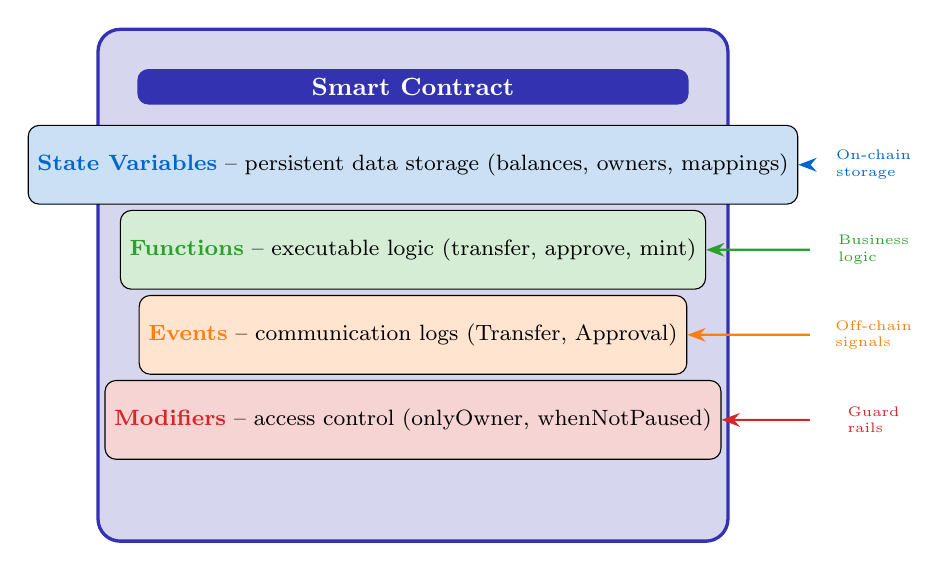
\begin{tikzpicture}[scale=0.9]
  % Outer contract box
  \node[draw,very thick,mlpurple,rounded corners=8pt,
        minimum width=8.0cm,minimum height=6.5cm,fill=mllavender4] (cbox) at (0,0) {};
  \node[fill=mlpurple,text=white,rounded corners=4pt,font=\small\bfseries,
        minimum width=7.0cm,align=center] at (0,2.8) {Smart Contract};

  % State Variables section
  \node[draw,fill=mlblue!20,rounded corners=4pt,
        minimum width=6.4cm,minimum height=1.0cm,align=center,font=\footnotesize]
        (sv) at (0,1.7) {\textbf{\textcolor{mlblue}{State Variables}} -- persistent data storage (balances, owners, mappings)};

  % Functions section
  \node[draw,fill=mlgreen!20,rounded corners=4pt,
        minimum width=6.4cm,minimum height=1.0cm,align=center,font=\footnotesize]
        (fn) at (0,0.5) {\textbf{\textcolor{mlgreen}{Functions}} -- executable logic (transfer, approve, mint)};

  % Events section
  \node[draw,fill=mlorange!20,rounded corners=4pt,
        minimum width=6.4cm,minimum height=1.0cm,align=center,font=\footnotesize]
        (ev) at (0,-0.7) {\textbf{\textcolor{mlorange}{Events}} -- communication logs (Transfer, Approval)};

  % Modifiers section
  \node[draw,fill=mlred!20,rounded corners=4pt,
        minimum width=6.4cm,minimum height=1.0cm,align=center,font=\footnotesize]
        (md) at (0,-1.9) {\textbf{\textcolor{mlred}{Modifiers}} -- access control (onlyOwner, whenNotPaused)};

  % Annotations on the right
  \node[font=\tiny,align=left,text=mlblue] at (6.5,1.7) {On-chain\\storage};
  \node[font=\tiny,align=left,text=mlgreen] at (6.5,0.5) {Business\\logic};
  \node[font=\tiny,align=left,text=mlorange] at (6.5,-0.7) {Off-chain\\signals};
  \node[font=\tiny,align=left,text=mlred] at (6.5,-1.9) {Guard\\rails};

  % Arrows from annotations
  \draw[-{Stealth},thick,mlblue] (5.6,1.7) -- (sv.east);
  \draw[-{Stealth},thick,mlgreen] (5.6,0.5) -- (fn.east);
  \draw[-{Stealth},thick,mlorange] (5.6,-0.7) -- (ev.east);
  \draw[-{Stealth},thick,mlred] (5.6,-1.9) -- (md.east);
\end{tikzpicture}
\vspace{2mm}
\begin{columns}[T]
\column{0.5\textwidth}
\begin{block}{Key Insight}
\footnotesize
Every smart contract is a combination of \textbf{data} (state variables) and \textbf{behavior} (functions), secured by \textbf{access rules} (modifiers) and broadcasting \textbf{outcomes} (events).
\end{block}
\column{0.5\textwidth}
\begin{exampleblock}{Think of It As\ldots}
\footnotesize
A class in object-oriented programming, but deployed on a global, immutable computer where every method call costs real money.
\end{exampleblock}
\end{columns}
\bottomnote{Smart contracts combine data storage, executable logic, access control, and event communication into a single on-chain program}
\end{frame}

% Frame 40: Smart Contract Lifecycle
\begin{frame}{Smart Contract Lifecycle}
\centering
\vspace{2mm}
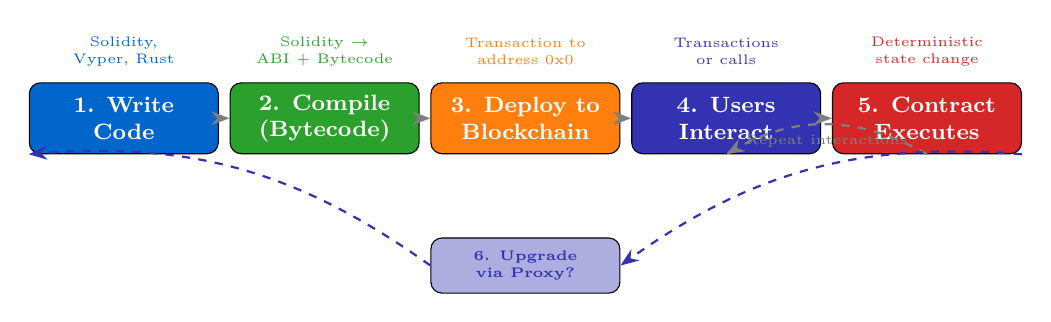
\begin{tikzpicture}[scale=0.85]
  % Step 1: Write Code
  \node[draw,fill=mlblue,text=white,rounded corners=4pt,
        minimum width=2.4cm,minimum height=0.9cm,align=center,font=\footnotesize\bfseries]
        (s1) at (0,0) {1. Write\\Code};
  % Step 2: Compile
  \node[draw,fill=mlgreen,text=white,rounded corners=4pt,
        minimum width=2.4cm,minimum height=0.9cm,align=center,font=\footnotesize\bfseries]
        (s2) at (3.0,0) {2. Compile\\(Bytecode)};
  % Step 3: Deploy
  \node[draw,fill=mlorange,text=white,rounded corners=4pt,
        minimum width=2.4cm,minimum height=0.9cm,align=center,font=\footnotesize\bfseries]
        (s3) at (6.0,0) {3. Deploy to\\Blockchain};
  % Step 4: Users Interact
  \node[draw,fill=mlpurple,text=white,rounded corners=4pt,
        minimum width=2.4cm,minimum height=0.9cm,align=center,font=\footnotesize\bfseries]
        (s4) at (9.0,0) {4. Users\\Interact};
  % Step 5: Contract Executes
  \node[draw,fill=mlred,text=white,rounded corners=4pt,
        minimum width=2.4cm,minimum height=0.9cm,align=center,font=\footnotesize\bfseries]
        (s5) at (12.0,0) {5. Contract\\Executes};

  % Arrows between steps
  \draw[-{Stealth},thick,mlgray] (s1.east) -- (s2.west);
  \draw[-{Stealth},thick,mlgray] (s2.east) -- (s3.west);
  \draw[-{Stealth},thick,mlgray] (s3.east) -- (s4.west);
  \draw[-{Stealth},thick,mlgray] (s4.east) -- (s5.west);

  % Feedback loop
  \draw[-{Stealth},thick,mlgray,dashed] (s5.south) to[bend right=30]
        node[midway,below,font=\tiny,text=mlgray,align=center] {Repeat interactions} (s4.south);

  % Upgrade path
  \node[draw,fill=mllavender,text=mlpurple,rounded corners=4pt,
        minimum width=2.4cm,minimum height=0.7cm,align=center,font=\tiny\bfseries]
        (up) at (6.0,-2.2) {6. Upgrade\\via Proxy?};
  \draw[-{Stealth},thick,mlpurple,dashed] (s5.south east) to[bend right=20] (up.east);
  \draw[-{Stealth},thick,mlpurple,dashed] (up.west) to[bend right=20] (s1.south west);

  % Annotations above
  \node[font=\tiny,text=mlblue,align=center] at (0,1.0) {Solidity,\\Vyper, Rust};
  \node[font=\tiny,text=mlgreen,align=center] at (3.0,1.0) {Solidity $\rightarrow$\\ABI + Bytecode};
  \node[font=\tiny,text=mlorange,align=center] at (6.0,1.0) {Transaction to\\address 0x0};
  \node[font=\tiny,text=mlpurple,align=center] at (9.0,1.0) {Transactions\\or calls};
  \node[font=\tiny,text=mlred,align=center] at (12.0,1.0) {Deterministic\\state change};
\end{tikzpicture}
\vspace{4mm}
\begin{columns}[T]
\column{0.5\textwidth}
\begin{block}{Deployment Details}
\footnotesize
\begin{itemize}
  \item Deployment is a special transaction to the zero address
  \item The contract receives a unique address (derived from deployer + nonce)
  \item Constructor runs once, initializing state
  \item Bytecode is stored immutably on-chain
\end{itemize}
\end{block}
\column{0.5\textwidth}
\begin{block}{After Deployment}
\footnotesize
\begin{itemize}
  \item Anyone with the address can interact
  \item Each interaction is a transaction (costs gas)
  \item Contract cannot be deleted (only self-destruct, now deprecated)
  \item Upgrade requires proxy patterns (see Frame 52)
\end{itemize}
\end{block}
\end{columns}
\bottomnote{Deployment is irreversible -- once bytecode is on-chain, the contract lives as long as the blockchain exists; upgrades require deliberate architectural patterns}
\end{frame}

% Frame 41: The Ethereum Virtual Machine Simplified
\begin{frame}{The Ethereum Virtual Machine Simplified}
\centering
\vspace{2mm}
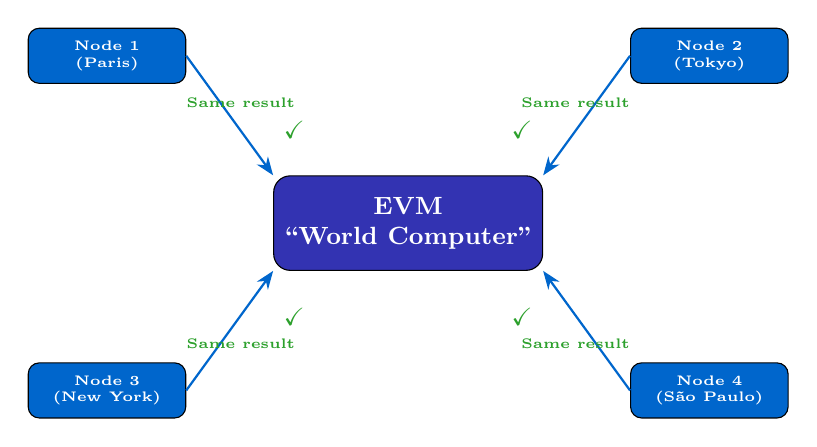
\begin{tikzpicture}[scale=0.85]
  % Central EVM node
  \node[draw,fill=mlpurple,text=white,rounded corners=6pt,
        minimum width=3.2cm,minimum height=1.2cm,align=center,font=\small\bfseries]
        (evm) at (6.0,0) {EVM\\``World Computer''};

  % Network nodes around it
  \node[draw,fill=mlblue,text=white,rounded corners=4pt,
        minimum width=2.0cm,minimum height=0.7cm,align=center,font=\tiny\bfseries]
        (n1) at (1.5,2.5) {Node 1\\(Paris)};
  \node[draw,fill=mlblue,text=white,rounded corners=4pt,
        minimum width=2.0cm,minimum height=0.7cm,align=center,font=\tiny\bfseries]
        (n2) at (10.5,2.5) {Node 2\\(Tokyo)};
  \node[draw,fill=mlblue,text=white,rounded corners=4pt,
        minimum width=2.0cm,minimum height=0.7cm,align=center,font=\tiny\bfseries]
        (n3) at (1.5,-2.5) {Node 3\\(New York)};
  \node[draw,fill=mlblue,text=white,rounded corners=4pt,
        minimum width=2.0cm,minimum height=0.7cm,align=center,font=\tiny\bfseries]
        (n4) at (10.5,-2.5) {Node 4\\(S\~{a}o Paulo)};

  % Arrows from nodes to EVM
  \draw[-{Stealth},thick,mlblue] (n1.east) -- (evm.north west);
  \draw[-{Stealth},thick,mlblue] (n2.west) -- (evm.north east);
  \draw[-{Stealth},thick,mlblue] (n3.east) -- (evm.south west);
  \draw[-{Stealth},thick,mlblue] (n4.west) -- (evm.south east);

  % Same result labels
  \node[font=\tiny\bfseries,text=mlgreen] at (3.5,1.8) {Same result};
  \node[font=\tiny\bfseries,text=mlgreen] at (8.5,1.8) {Same result};
  \node[font=\tiny\bfseries,text=mlgreen] at (3.5,-1.8) {Same result};
  \node[font=\tiny\bfseries,text=mlgreen] at (8.5,-1.8) {Same result};

  % Checkmarks
  \node[font=\small,text=mlgreen] at (4.3,1.4) {\checkmark};
  \node[font=\small,text=mlgreen] at (7.7,1.4) {\checkmark};
  \node[font=\small,text=mlgreen] at (4.3,-1.4) {\checkmark};
  \node[font=\small,text=mlgreen] at (7.7,-1.4) {\checkmark};
\end{tikzpicture}
\vspace{3mm}
\begin{columns}[T]
\column{0.33\textwidth}
\begin{block}{\textcolor{mlblue}{Global Computer}}
\footnotesize
\begin{itemize}
  \item Shared by all Ethereum nodes
  \item Every node runs the \emph{same} computation
  \item State stored across the entire network
\end{itemize}
\end{block}
\column{0.33\textwidth}
\begin{block}{\textcolor{mlgreen}{Deterministic}}
\footnotesize
\begin{itemize}
  \item Same input always yields same output
  \item No randomness, no external calls during execution
  \item Consensus ensures agreement
\end{itemize}
\end{block}
\column{0.33\textwidth}
\begin{block}{\textcolor{mlorange}{Stack-Based}}
\footnotesize
\begin{itemize}
  \item 256-bit word size (optimized for cryptography)
  \item Opcodes: ADD, MUL, SSTORE, CALL, etc.
  \item Turing-complete (with gas limit)
\end{itemize}
\end{block}
\end{columns}
\bottomnote{The EVM is often called the ``world computer'' -- a single virtual machine replicated across thousands of nodes, ensuring trustless, deterministic execution}
\end{frame}

% Frame 42: Gas: Paying for Computation
\begin{frame}{Gas: Paying for Computation}
\begin{columns}[T]
\column{0.5\textwidth}
\begin{block}{Why Gas Exists}
\footnotesize
\begin{itemize}
  \item \textbf{Prevents infinite loops} -- every operation has a cost; programs that run too long simply run out of gas
  \item \textbf{Compensates validators} -- miners/validators earn fees for processing transactions
  \item \textbf{Market-based pricing} -- gas price fluctuates with network demand
  \item \textbf{Resource allocation} -- scarce block space is allocated to those willing to pay
\end{itemize}
\end{block}
\vspace{2mm}
\begin{exampleblock}{Simple Example}
\footnotesize
\begin{itemize}
  \item Sending ETH costs \textbf{21,000 gas} (base)
  \item At 30 Gwei gas price: $21{,}000 \times 30 = 630{,}000$ Gwei
  \item That is \textbf{0.00063 ETH} $\approx$ \$2--3
\end{itemize}
\end{exampleblock}

\column{0.5\textwidth}
\begin{block}{Gas Fee Formula}
\footnotesize
\centering
\vspace{2mm}
\textcolor{mlpurple}{\textbf{Total Fee = Gas Used $\times$ Gas Price}}
\vspace{3mm}

\begin{tabular}{l r}
\toprule
\textbf{Operation} & \textbf{Gas Cost} \\
\midrule
\rowcolor{mllavender4}
ETH transfer & 21,000 \\
ERC-20 transfer & \textasciitilde65,000 \\
\rowcolor{mllavender4}
Uniswap swap & \textasciitilde150,000 \\
NFT mint & \textasciitilde200,000 \\
\rowcolor{mllavender4}
Contract deploy & 1M--5M \\
\bottomrule
\end{tabular}
\end{block}
\vspace{2mm}
\begin{alertblock}{EIP-1559 (Since Aug 2021)}
\footnotesize
Base fee is \textbf{burned} (deflationary), priority fee goes to validators. Users set a max fee; unused gas is refunded.
\end{alertblock}
\end{columns}
\bottomnote{Gas is the fundamental economic mechanism preventing abuse of the shared EVM -- every computation costs real money, aligning incentives across the network}
\end{frame}

% Frame 43: Reading vs Writing: Free vs Paid
\begin{frame}{Reading vs Writing: Free vs Paid}
\begin{columns}[T]
\column{0.48\textwidth}
\begin{block}{\textcolor{mlgreen}{FREE -- Read Operations}}
\footnotesize
\begin{itemize}
  \item \textbf{View functions} -- read state without modifying it
  \item \textbf{Pure functions} -- compute results from inputs only
  \item \textbf{Querying balances} -- check token holdings
  \item \textbf{Reading mappings} -- look up stored values
  \item \textbf{Calling constants} -- retrieve fixed parameters
\end{itemize}
\vspace{2mm}
\centering
\textcolor{mlgreen}{\textbf{No transaction needed}}\\
\footnotesize Executed locally by your node
\end{block}

\column{0.48\textwidth}
\begin{alertblock}{\textcolor{mlred}{COSTS GAS -- Write Operations}}
\footnotesize
\begin{itemize}
  \item \textbf{State changes} -- updating stored variables
  \item \textbf{Token transfers} -- moving ERC-20 or ERC-721 tokens
  \item \textbf{Contract calls} -- invoking functions that modify state
  \item \textbf{Emitting events} -- writing to transaction logs
  \item \textbf{Creating contracts} -- deploying new contracts
\end{itemize}
\vspace{2mm}
\centering
\textcolor{mlred}{\textbf{Transaction required}}\\
\footnotesize Processed by all validators
\end{alertblock}
\end{columns}
\vspace{3mm}
\centering
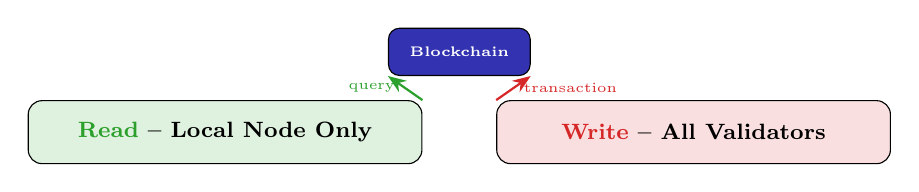
\begin{tikzpicture}[scale=0.85]
  \node[draw,fill=mlgreen!15,rounded corners=5pt,
        minimum width=5.0cm,minimum height=0.8cm,align=center,font=\footnotesize\bfseries]
        (rd) at (-3.5,0) {\textcolor{mlgreen}{Read} -- Local Node Only};
  \node[draw,fill=mlred!15,rounded corners=5pt,
        minimum width=5.0cm,minimum height=0.8cm,align=center,font=\footnotesize\bfseries]
        (wr) at (3.5,0) {\textcolor{mlred}{Write} -- All Validators};
  \node[draw,fill=mlpurple,text=white,rounded corners=4pt,
        minimum width=1.8cm,minimum height=0.6cm,align=center,font=\tiny\bfseries]
        (bc) at (0,1.2) {Blockchain};
  \draw[-{Stealth},thick,mlgreen] (rd.north east) -- (bc.south west)
        node[midway,left,font=\tiny,text=mlgreen] {query};
  \draw[-{Stealth},thick,mlred] (wr.north west) -- (bc.south east)
        node[midway,right,font=\tiny,text=mlred] {transaction};
\end{tikzpicture}
\bottomnote{Understanding the read/write distinction is essential for cost-effective dApp design -- minimize state changes to reduce gas consumption}
\end{frame}

% Frame 44: Events and Logging
\begin{frame}{Events and Logging}
\begin{columns}[T]
\column{0.5\textwidth}
\begin{block}{What Are Events?}
\footnotesize
Events are signals \textbf{emitted during contract execution}:
\begin{itemize}
  \item Stored in \textbf{transaction logs}, not contract state
  \item Cannot be read by other smart contracts
  \item Accessible to off-chain applications (dApps, indexers)
  \item Up to 3 \textbf{indexed} parameters for efficient filtering
\end{itemize}
\end{block}
\vspace{2mm}
\begin{block}{Why Use Events?}
\footnotesize
\begin{itemize}
  \item \textbf{Much cheaper} than storage writes (\textasciitilde375 gas per log byte vs.\ 20,000 gas per storage slot)
  \item \textbf{Real-time updates} for frontend UIs
  \item \textbf{Historical record} queryable via block explorers
  \item \textbf{The Graph protocol} indexes events into queryable APIs
\end{itemize}
\end{block}

\column{0.5\textwidth}
\centering
\vspace{2mm}
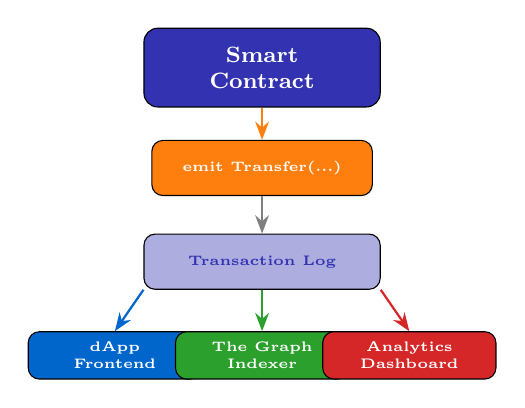
\begin{tikzpicture}[scale=0.85]
  % Smart Contract
  \node[draw,fill=mlpurple,text=white,rounded corners=5pt,
        minimum width=3.0cm,minimum height=1.0cm,align=center,font=\footnotesize\bfseries]
        (sc) at (0,3.5) {Smart\\Contract};

  % Emit event
  \node[draw,fill=mlorange,text=white,rounded corners=4pt,
        minimum width=2.8cm,minimum height=0.7cm,align=center,font=\tiny\bfseries]
        (em) at (0,2.0) {emit Transfer(...)};

  % Transaction log
  \node[draw,fill=mllavender,text=mlpurple,rounded corners=4pt,
        minimum width=3.0cm,minimum height=0.7cm,align=center,font=\tiny\bfseries]
        (log) at (0,0.6) {Transaction Log};

  % Consumers
  \node[draw,fill=mlblue,text=white,rounded corners=4pt,
        minimum width=2.2cm,minimum height=0.6cm,align=center,font=\tiny\bfseries]
        (d1) at (-2.2,-0.8) {dApp\\Frontend};
  \node[draw,fill=mlgreen,text=white,rounded corners=4pt,
        minimum width=2.2cm,minimum height=0.6cm,align=center,font=\tiny\bfseries]
        (d2) at (0,-0.8) {The Graph\\Indexer};
  \node[draw,fill=mlred,text=white,rounded corners=4pt,
        minimum width=2.2cm,minimum height=0.6cm,align=center,font=\tiny\bfseries]
        (d3) at (2.2,-0.8) {Analytics\\Dashboard};

  % Arrows
  \draw[-{Stealth},thick,mlorange] (sc.south) -- (em.north);
  \draw[-{Stealth},thick,mlgray] (em.south) -- (log.north);
  \draw[-{Stealth},thick,mlblue] (log.south west) -- (d1.north);
  \draw[-{Stealth},thick,mlgreen] (log.south) -- (d2.north);
  \draw[-{Stealth},thick,mlred] (log.south east) -- (d3.north);
\end{tikzpicture}
\vspace{2mm}
\begin{exampleblock}{Common Events}
\footnotesize
\texttt{Transfer(from, to, amount)} -- ERC-20 transfers\\
\texttt{Approval(owner, spender, amount)} -- spending allowances\\
\texttt{Swap(sender, amountIn, amountOut)} -- DEX trades
\end{exampleblock}
\end{columns}
\bottomnote{Events are the primary communication channel between smart contracts and the outside world -- they power real-time dApp interfaces and blockchain analytics}
\end{frame}

% Frame 45: Oracles: Connecting to the Real World
\begin{frame}{Oracles: Connecting to the Real World}
\centering
\vspace{2mm}
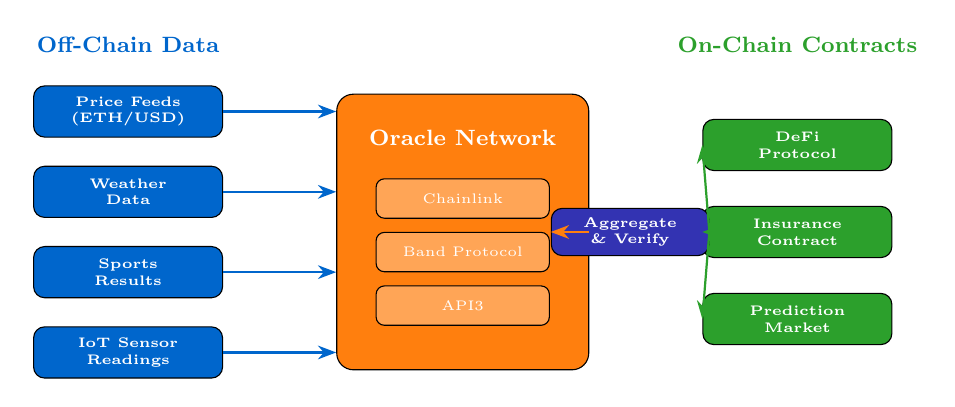
\begin{tikzpicture}[scale=0.85]
  % Off-chain data sources (left)
  \node[draw,fill=mlblue,text=white,rounded corners=4pt,
        minimum width=2.4cm,minimum height=0.65cm,align=center,font=\tiny\bfseries]
        (ds1) at (0,2.0) {Price Feeds\\(ETH/USD)};
  \node[draw,fill=mlblue,text=white,rounded corners=4pt,
        minimum width=2.4cm,minimum height=0.65cm,align=center,font=\tiny\bfseries]
        (ds2) at (0,0.8) {Weather\\Data};
  \node[draw,fill=mlblue,text=white,rounded corners=4pt,
        minimum width=2.4cm,minimum height=0.65cm,align=center,font=\tiny\bfseries]
        (ds3) at (0,-0.4) {Sports\\Results};
  \node[draw,fill=mlblue,text=white,rounded corners=4pt,
        minimum width=2.4cm,minimum height=0.65cm,align=center,font=\tiny\bfseries]
        (ds4) at (0,-1.6) {IoT Sensor\\Readings};

  % Off-chain label
  \node[font=\footnotesize\bfseries,text=mlblue] at (0,3.0) {Off-Chain Data};

  % Oracle network (middle)
  \node[draw,fill=mlorange,text=white,rounded corners=6pt,
        minimum width=3.2cm,minimum height=3.5cm,align=center] (obox) at (5.0,0.2) {};
  \node[fill=mlorange,text=white,rounded corners=4pt,font=\footnotesize\bfseries,
        minimum width=2.8cm,align=center] at (5.0,1.6) {Oracle Network};
  \node[draw,fill=mlorange!70,text=white,rounded corners=3pt,
        minimum width=2.2cm,minimum height=0.5cm,align=center,font=\tiny]
        (o1) at (5.0,0.7) {Chainlink};
  \node[draw,fill=mlorange!70,text=white,rounded corners=3pt,
        minimum width=2.2cm,minimum height=0.5cm,align=center,font=\tiny]
        (o2) at (5.0,-0.1) {Band Protocol};
  \node[draw,fill=mlorange!70,text=white,rounded corners=3pt,
        minimum width=2.2cm,minimum height=0.5cm,align=center,font=\tiny]
        (o3) at (5.0,-0.9) {API3};

  % On-chain smart contracts (right)
  \node[draw,fill=mlgreen,text=white,rounded corners=4pt,
        minimum width=2.4cm,minimum height=0.65cm,align=center,font=\tiny\bfseries]
        (sc1) at (10.0,1.5) {DeFi\\Protocol};
  \node[draw,fill=mlgreen,text=white,rounded corners=4pt,
        minimum width=2.4cm,minimum height=0.65cm,align=center,font=\tiny\bfseries]
        (sc2) at (10.0,0.2) {Insurance\\Contract};
  \node[draw,fill=mlgreen,text=white,rounded corners=4pt,
        minimum width=2.4cm,minimum height=0.65cm,align=center,font=\tiny\bfseries]
        (sc3) at (10.0,-1.1) {Prediction\\Market};

  % On-chain label
  \node[font=\footnotesize\bfseries,text=mlgreen] at (10.0,3.0) {On-Chain Contracts};

  % Aggregation node
  \node[draw,fill=mlpurple,text=white,rounded corners=4pt,
        minimum width=2.0cm,minimum height=0.6cm,align=center,font=\tiny\bfseries]
        (agg) at (7.5,0.2) {Aggregate\\\& Verify};

  % Arrows: data sources to oracle network
  \draw[-{Stealth},thick,mlblue] (ds1.east) -- (obox.west |- ds1);
  \draw[-{Stealth},thick,mlblue] (ds2.east) -- (obox.west |- ds2);
  \draw[-{Stealth},thick,mlblue] (ds3.east) -- (obox.west |- ds3);
  \draw[-{Stealth},thick,mlblue] (ds4.east) -- (obox.west |- ds4);

  % Arrows: oracle to aggregation
  \draw[-{Stealth},thick,mlorange] (obox.east) -- (agg.west);

  % Arrows: aggregation to smart contracts
  \draw[-{Stealth},thick,mlgreen] (agg.east) -- (sc1.west);
  \draw[-{Stealth},thick,mlgreen] (agg.east) -- (sc2.west);
  \draw[-{Stealth},thick,mlgreen] (agg.east) -- (sc3.west);
\end{tikzpicture}
\vspace{3mm}
\begin{columns}[T]
\column{0.5\textwidth}
\begin{block}{The Oracle Problem}
\footnotesize
Blockchains are \textbf{deterministic and isolated} -- they cannot access external data on their own. Oracles provide a trusted bridge, but introduce centralization risk.
\end{block}
\column{0.5\textwidth}
\begin{block}{Chainlink Dominance}
\footnotesize
\begin{itemize}
  \item Secures \textasciitilde\$75B+ in DeFi TVL
  \item 1,700+ integrations across 30+ chains
  \item Decentralized oracle network with staking
  \item CCIP for cross-chain communication
\end{itemize}
\end{block}
\end{columns}
\bottomnote{Chainlink is the dominant oracle network, securing the majority of DeFi -- the oracle problem remains one of the most critical challenges in blockchain design}
\end{frame}

% Frame 46: Token Standards Overview
\begin{frame}{Token Standards Overview}
\begin{columns}[T]
\column{0.33\textwidth}
\begin{block}{\textcolor{mlblue}{ERC-20 (Fungible)}}
\footnotesize
\begin{itemize}
  \item Every token is \textbf{identical} and interchangeable
  \item Examples: USDT, LINK, UNI, AAVE
  \item Functions: \texttt{transfer}, \texttt{approve}, \texttt{balanceOf}
  \item Most widely adopted standard
  \item Powers all DeFi liquidity
\end{itemize}
\vspace{1mm}
\centering
\textcolor{mlblue}{\textbf{Think: dollar bills}}
\end{block}

\column{0.33\textwidth}
\begin{block}{\textcolor{mlgreen}{ERC-721 (NFT)}}
\footnotesize
\begin{itemize}
  \item Each token is \textbf{unique} with a distinct ID
  \item Examples: CryptoPunks, BAYC, ENS names
  \item Functions: \texttt{ownerOf}, \texttt{tokenURI}, \texttt{safeTransferFrom}
  \item Metadata links to art, music, or documents
  \item Provable digital ownership
\end{itemize}
\vspace{1mm}
\centering
\textcolor{mlgreen}{\textbf{Think: concert tickets}}
\end{block}

\column{0.33\textwidth}
\begin{block}{\textcolor{mlorange}{ERC-1155 (Multi)}}
\footnotesize
\begin{itemize}
  \item Supports \textbf{both} fungible and non-fungible in one contract
  \item Examples: gaming items, batch collectibles
  \item Functions: \texttt{balanceOf}, \texttt{safeBatchTransferFrom}
  \item Gas-efficient batch operations
  \item One contract for many token types
\end{itemize}
\vspace{1mm}
\centering
\textcolor{mlorange}{\textbf{Think: game inventory}}
\end{block}
\end{columns}
\vspace{3mm}
\centering
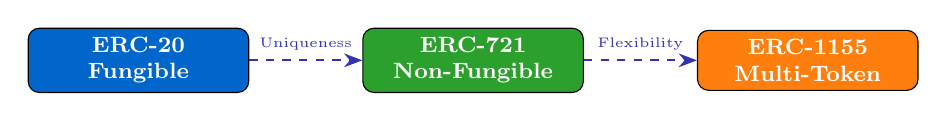
\begin{tikzpicture}[scale=0.85]
  \node[draw,fill=mlblue,text=white,rounded corners=4pt,
        minimum width=2.8cm,minimum height=0.7cm,align=center,font=\footnotesize\bfseries]
        (e20) at (0,0) {ERC-20\\Fungible};
  \node[draw,fill=mlgreen,text=white,rounded corners=4pt,
        minimum width=2.8cm,minimum height=0.7cm,align=center,font=\footnotesize\bfseries]
        (e721) at (5.0,0) {ERC-721\\Non-Fungible};
  \node[draw,fill=mlorange,text=white,rounded corners=4pt,
        minimum width=2.8cm,minimum height=0.7cm,align=center,font=\footnotesize\bfseries]
        (e1155) at (10.0,0) {ERC-1155\\Multi-Token};
  \draw[-{Stealth},thick,mlpurple,dashed] (e20.east) -- (e721.west)
        node[midway,above,font=\tiny,text=mlpurple] {Uniqueness};
  \draw[-{Stealth},thick,mlpurple,dashed] (e721.east) -- (e1155.west)
        node[midway,above,font=\tiny,text=mlpurple] {Flexibility};
\end{tikzpicture}
\bottomnote{Token standards enable composability -- any ERC-20 token works with any DEX, any ERC-721 works with any NFT marketplace, creating a permissionless ecosystem}
\end{frame}

%% ============================================================
%% SECTION 5: APPLICATIONS, SECURITY, AND FUTURE
%% ============================================================
\section{Applications, Security, and Future}

% Frame 47: Decentralized Exchanges
\begin{frame}{Decentralized Exchanges}
\begin{columns}[T]
\column{0.5\textwidth}
\begin{block}{Automated Market Makers (AMMs)}
\footnotesize
Traditional exchanges use \textbf{order books}; DEXs use \textbf{liquidity pools}:
\begin{itemize}
  \item Paired tokens locked in a smart contract pool
  \item Price determined by the ratio of tokens in the pool
  \item \textbf{Constant product formula}: $x \times y = k$
  \item Anyone can provide liquidity and earn trading fees
  \item No registration, no KYC, no counterparty risk
\end{itemize}
\end{block}
\vspace{2mm}
\begin{exampleblock}{Top DEXs by Volume}
\footnotesize
\begin{itemize}
  \item \textbf{Uniswap}: \textasciitilde\$1T+ cumulative volume, Ethereum pioneer
  \item \textbf{Curve}: Optimized for stablecoin swaps (low slippage)
  \item \textbf{SushiSwap}: Multi-chain, community-governed
  \item \textbf{PancakeSwap}: BNB Chain, low fees
\end{itemize}
\end{exampleblock}

\column{0.5\textwidth}
\centering
\vspace{2mm}
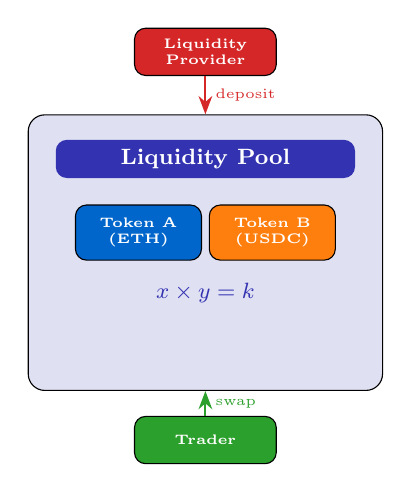
\begin{tikzpicture}[scale=0.85]
  % Liquidity Pool
  \node[draw,fill=mlpurple!15,rounded corners=6pt,
        minimum width=4.5cm,minimum height=3.5cm] (pool) at (0,0) {};
  \node[fill=mlpurple,text=white,rounded corners=4pt,font=\footnotesize\bfseries,
        minimum width=3.8cm,align=center] at (0,1.4) {Liquidity Pool};

  % Token A
  \node[draw,fill=mlblue,text=white,rounded corners=4pt,
        minimum width=1.6cm,minimum height=0.7cm,align=center,font=\tiny\bfseries]
        (ta) at (-1.0,0.3) {Token A\\(ETH)};
  % Token B
  \node[draw,fill=mlorange,text=white,rounded corners=4pt,
        minimum width=1.6cm,minimum height=0.7cm,align=center,font=\tiny\bfseries]
        (tb) at (1.0,0.3) {Token B\\(USDC)};

  % Formula
  \node[font=\footnotesize\bfseries,text=mlpurple] at (0,-0.6) {$x \times y = k$};

  % Trader
  \node[draw,fill=mlgreen,text=white,rounded corners=4pt,
        minimum width=1.8cm,minimum height=0.6cm,align=center,font=\tiny\bfseries]
        (tr) at (0,-2.8) {Trader};

  % LP
  \node[draw,fill=mlred,text=white,rounded corners=4pt,
        minimum width=1.8cm,minimum height=0.6cm,align=center,font=\tiny\bfseries]
        (lp) at (0,3.0) {Liquidity\\Provider};

  % Arrows
  \draw[-{Stealth},thick,mlgreen] (tr.north) -- (pool.south)
        node[midway,right,font=\tiny,text=mlgreen] {swap};
  \draw[-{Stealth},thick,mlred] (lp.south) -- (pool.north)
        node[midway,right,font=\tiny,text=mlred] {deposit};
\end{tikzpicture}
\vspace{2mm}
\begin{alertblock}{Impermanent Loss}
\footnotesize
LPs face loss when token prices diverge -- the pool rebalances against them. Fees may or may not compensate.
\end{alertblock}
\end{columns}
\bottomnote{AMMs replaced order books with mathematical formulas, enabling trustless 24/7 trading without intermediaries -- Uniswap alone processes billions in weekly volume}
\end{frame}

% Frame 48: Lending Protocols
\begin{frame}{Lending Protocols}
\begin{columns}[T]
\column{0.5\textwidth}
\begin{block}{How Aave/Compound Work}
\footnotesize
\begin{enumerate}
  \item \textbf{Deposit assets} $\rightarrow$ earn variable interest
  \item \textbf{Borrow against collateral} $\rightarrow$ over-collateralized loans (e.g., deposit \$150 ETH, borrow \$100 USDC)
  \item \textbf{Interest accrues} $\rightarrow$ rates set by supply/demand algorithms
  \item \textbf{Liquidation} $\rightarrow$ if collateral value drops below threshold, anyone can repay the debt and claim collateral at a discount
\end{enumerate}
\end{block}
\vspace{2mm}
\begin{exampleblock}{Key Metrics}
\footnotesize
\begin{itemize}
  \item Aave: \textasciitilde\$10B+ TVL across 7 chains
  \item Compound: Pioneer of algorithmic interest rates
  \item MakerDAO: \textasciitilde\$8B+ in collateral backing DAI
\end{itemize}
\end{exampleblock}

\column{0.5\textwidth}
\begin{block}{Flash Loans: Borrow Without Collateral}
\footnotesize
A unique DeFi primitive:
\begin{itemize}
  \item Borrow \textbf{any amount} with \textbf{zero collateral}
  \item Must \textbf{repay in the same transaction}
  \item If not repaid $\rightarrow$ entire transaction reverts (atomicity)
  \item Use cases: arbitrage, collateral swaps, liquidations
\end{itemize}
\end{block}
\vspace{2mm}
\centering
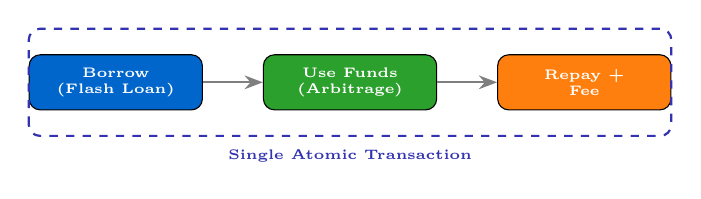
\begin{tikzpicture}[scale=0.85]
  \node[draw,fill=mlblue,text=white,rounded corners=4pt,
        minimum width=2.2cm,minimum height=0.7cm,align=center,font=\tiny\bfseries]
        (borrow) at (0,0) {Borrow\\(Flash Loan)};
  \node[draw,fill=mlgreen,text=white,rounded corners=4pt,
        minimum width=2.2cm,minimum height=0.7cm,align=center,font=\tiny\bfseries]
        (use) at (3.5,0) {Use Funds\\(Arbitrage)};
  \node[draw,fill=mlorange,text=white,rounded corners=4pt,
        minimum width=2.2cm,minimum height=0.7cm,align=center,font=\tiny\bfseries]
        (repay) at (7.0,0) {Repay +\\Fee};
  \draw[-{Stealth},thick,mlgray] (borrow.east) -- (use.west);
  \draw[-{Stealth},thick,mlgray] (use.east) -- (repay.west);

  % All in one tx
  \draw[thick,mlpurple,dashed,rounded corners=4pt]
        (-1.3,-0.8) rectangle (8.3,0.8);
  \node[font=\tiny\bfseries,text=mlpurple] at (3.5,-1.1) {Single Atomic Transaction};
\end{tikzpicture}
\vspace{1mm}
\begin{alertblock}{Risk}
\footnotesize
Flash loans have been used in exploits -- attackers manipulate prices within a single transaction to drain protocols.
\end{alertblock}
\end{columns}
\bottomnote{DeFi lending removes banks from the equation -- algorithms set rates, smart contracts enforce rules, and liquidation is permissionless and instant}
\end{frame}

% Frame 49: Stablecoins as Smart Contracts
\begin{frame}{Stablecoins as Smart Contracts}
\begin{columns}[T]
\column{0.33\textwidth}
\begin{block}{\textcolor{mlblue}{Collateralized (DAI)}}
\footnotesize
\begin{itemize}
  \item \textbf{Over-collateralized} with ETH and other assets (150\%+)
  \item Governed by \textbf{MakerDAO} (decentralized)
  \item Users lock collateral in ``Vaults''
  \item Liquidation if collateral ratio drops
  \item Transparent, auditable on-chain
\end{itemize}
\vspace{1mm}
\centering
\textcolor{mlblue}{\textbf{Trustless, decentralized}}
\end{block}

\column{0.33\textwidth}
\begin{block}{\textcolor{mlorange}{Centralized (USDC/USDT)}}
\footnotesize
\begin{itemize}
  \item Backed by \textbf{fiat reserves} (cash, T-bills)
  \item Issued by centralized entities (Circle, Tether)
  \item Smart contract handles \textbf{transfers only}
  \item \textbf{Blacklist function} -- issuer can freeze addresses
  \item Monthly attestations (not full audits)
\end{itemize}
\vspace{1mm}
\centering
\textcolor{mlorange}{\textbf{Centralized trust}}
\end{block}

\column{0.33\textwidth}
\begin{block}{\textcolor{mlred}{Algorithmic (Historical)}}
\footnotesize
\begin{itemize}
  \item \textbf{Mint/burn mechanism} to maintain \$1 peg
  \item No backing -- relies on arbitrage incentives
  \item \textbf{Terra/UST collapse} (May 2022): \$40B+ wiped out
  \item ``Death spiral'' when confidence breaks
  \item Largely discredited as standalone model
\end{itemize}
\vspace{1mm}
\centering
\textcolor{mlred}{\textbf{High risk, mostly failed}}
\end{block}
\end{columns}
\vspace{3mm}
\centering
\footnotesize
\begin{tabular}{l c c c}
\toprule
\textbf{Feature} & \textbf{DAI} & \textbf{USDC} & \textbf{Algo (UST)} \\
\midrule
\rowcolor{mllavender4}
Backing & Crypto collateral & Fiat reserves & Algorithm \\
Decentralization & High & Low & Medium \\
\rowcolor{mllavender4}
Censorship resistance & High & Low (blacklist) & Medium \\
Peg stability & Strong & Very strong & Failed \\
\bottomrule
\end{tabular}
\bottomnote{Stablecoins are the backbone of DeFi -- understanding their trust assumptions (collateral vs.\ reserves vs.\ algorithms) is critical for risk assessment}
\end{frame}

% Frame 50: Smart Contract Security Best Practices
\begin{frame}{Smart Contract Security Best Practices}
\begin{columns}[T]
\column{0.5\textwidth}
\begin{block}{Pre-Deployment Checklist}
\footnotesize
\begin{enumerate}
  \item \textcolor{mlblue}{\textbf{Professional audits}} -- engage 2+ independent audit firms for critical protocols
  \item \textcolor{mlgreen}{\textbf{Formal verification}} -- mathematically prove critical invariants (Certora, Halmos)
  \item \textcolor{mlorange}{\textbf{Comprehensive testing}} -- unit, integration, fuzz, and invariant tests with $>$95\% coverage
  \item \textcolor{mlpurple}{\textbf{Time-tested libraries}} -- use OpenZeppelin for standard patterns (battle-tested by billions in TVL)
  \item \textcolor{mlred}{\textbf{Staged deployment}} -- testnet $\rightarrow$ limited mainnet $\rightarrow$ full launch with caps
\end{enumerate}
\end{block}

\column{0.5\textwidth}
\begin{block}{Post-Deployment Defense}
\footnotesize
\begin{enumerate}
  \item \textcolor{mlblue}{\textbf{Bug bounty programs}} -- Immunefi hosts bounties up to \$10M for critical bugs
  \item \textcolor{mlgreen}{\textbf{Monitoring and alerts}} -- real-time tracking of unusual transactions (Forta, Tenderly)
  \item \textcolor{mlorange}{\textbf{Incident response plan}} -- predefined procedures for emergency pausing and mitigation
  \item \textcolor{mlpurple}{\textbf{Timelock governance}} -- delay critical parameter changes (24--72 hours) to allow community review
  \item \textcolor{mlred}{\textbf{Circuit breakers}} -- automatic pause if TVL drops rapidly or anomalies detected
\end{enumerate}
\end{block}
\end{columns}
\vspace{3mm}
\centering
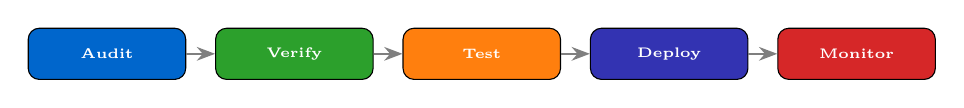
\begin{tikzpicture}[scale=0.85]
  \node[draw,fill=mlblue,text=white,rounded corners=4pt,
        minimum width=2.0cm,minimum height=0.65cm,align=center,font=\tiny\bfseries]
        (a1) at (0,0) {Audit};
  \node[draw,fill=mlgreen,text=white,rounded corners=4pt,
        minimum width=2.0cm,minimum height=0.65cm,align=center,font=\tiny\bfseries]
        (a2) at (2.8,0) {Verify};
  \node[draw,fill=mlorange,text=white,rounded corners=4pt,
        minimum width=2.0cm,minimum height=0.65cm,align=center,font=\tiny\bfseries]
        (a3) at (5.6,0) {Test};
  \node[draw,fill=mlpurple,text=white,rounded corners=4pt,
        minimum width=2.0cm,minimum height=0.65cm,align=center,font=\tiny\bfseries]
        (a4) at (8.4,0) {Deploy};
  \node[draw,fill=mlred,text=white,rounded corners=4pt,
        minimum width=2.0cm,minimum height=0.65cm,align=center,font=\tiny\bfseries]
        (a5) at (11.2,0) {Monitor};
  \draw[-{Stealth},thick,mlgray] (a1.east) -- (a2.west);
  \draw[-{Stealth},thick,mlgray] (a2.east) -- (a3.west);
  \draw[-{Stealth},thick,mlgray] (a3.east) -- (a4.west);
  \draw[-{Stealth},thick,mlgray] (a4.east) -- (a5.west);
\end{tikzpicture}
\bottomnote{Security is not a one-time event -- it is a continuous lifecycle from design through deployment and beyond; the cost of an audit is always less than the cost of an exploit}
\end{frame}

% Frame 51: Famous Smart Contract Failures
\begin{frame}{Famous Smart Contract Failures}
\centering
\vspace{2mm}
\footnotesize
\begin{tabular}{l l r l}
\toprule
\textbf{Year} & \textbf{Exploit} & \textbf{Loss} & \textbf{Root Cause} \\
\midrule
\rowcolor{mllavender4}
2016 & The DAO & \$60M & Reentrancy -- recursive withdrawal drained funds \\
2017 & Parity Wallet & \$150M & Unprotected \texttt{initWallet()} -- anyone could claim ownership \\
\rowcolor{mllavender4}
2020 & bZx Flash Loan & \$8M & Price oracle manipulation via flash loan \\
2021 & Poly Network & \$611M & Cross-chain signature verification bypass \\
\rowcolor{mllavender4}
2022 & Wormhole Bridge & \$320M & Signature verification bypass in bridge contract \\
2022 & Ronin Bridge & \$625M & 5 of 9 validator keys compromised (social engineering) \\
\rowcolor{mllavender4}
2022 & Terra/UST & \$40B+ & Algorithmic stablecoin death spiral \\
2023 & Euler Finance & \$197M & Donation attack exploiting accounting logic \\
\rowcolor{mllavender4}
2023 & Curve Finance & \$70M & Vyper compiler reentrancy bug \\
\bottomrule
\end{tabular}
\vspace{4mm}
\begin{columns}[T]
\column{0.5\textwidth}
\begin{block}{Common Vulnerability Patterns}
\footnotesize
\begin{itemize}
  \item \textcolor{mlred}{\textbf{Reentrancy}} -- calling external contracts before updating state
  \item \textcolor{mlorange}{\textbf{Access control}} -- missing or incorrect permission checks
  \item \textcolor{mlblue}{\textbf{Oracle manipulation}} -- exploiting price feed dependencies
\end{itemize}
\end{block}
\column{0.5\textwidth}
\begin{alertblock}{Key Lesson}
\footnotesize
Over \textbf{\$3 billion} has been lost to smart contract exploits. Every major failure has taught the ecosystem valuable lessons -- most could have been prevented by following known security practices.
\end{alertblock}
\end{columns}
\bottomnote{Each exploit advanced the industry -- The DAO led to reentrancy guards; Parity led to better access control; bridge hacks led to multi-sig improvements}
\end{frame}

% Frame 52: Upgradeability Patterns
\begin{frame}{Upgradeability Patterns}
\centering
\vspace{2mm}
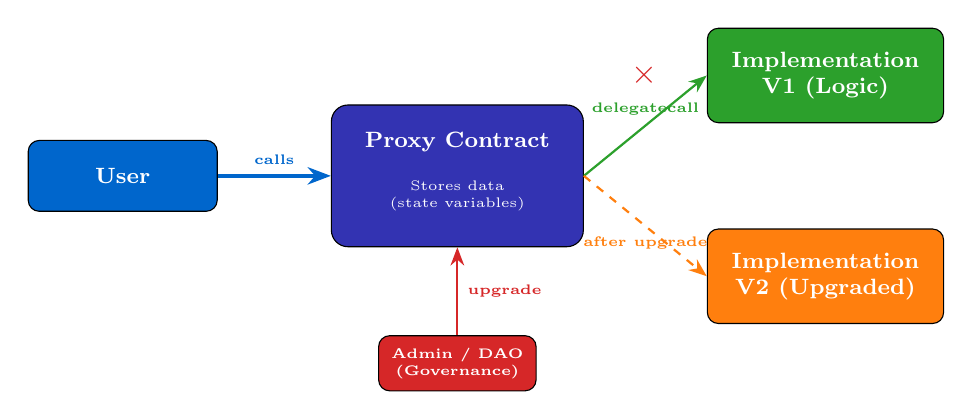
\begin{tikzpicture}[scale=0.85]
  % User
  \node[draw,fill=mlblue,text=white,rounded corners=4pt,
        minimum width=2.4cm,minimum height=0.9cm,align=center,font=\footnotesize\bfseries]
        (user) at (0,0) {User};

  % Proxy Contract
  \node[draw,fill=mlpurple,text=white,rounded corners=6pt,
        minimum width=3.2cm,minimum height=1.8cm,align=center] (proxy) at (5.0,0) {};
  \node[fill=mlpurple,text=white,rounded corners=4pt,font=\footnotesize\bfseries,
        minimum width=2.8cm,align=center] at (5.0,0.5) {Proxy Contract};
  \node[font=\tiny,text=white,align=center] at (5.0,-0.3) {Stores data\\(state variables)};

  % Implementation V1
  \node[draw,fill=mlgreen,text=white,rounded corners=4pt,
        minimum width=3.0cm,minimum height=1.2cm,align=center,font=\footnotesize\bfseries]
        (impl1) at (10.5,1.5) {Implementation\\V1 (Logic)};

  % Implementation V2
  \node[draw,fill=mlorange,text=white,rounded corners=4pt,
        minimum width=3.0cm,minimum height=1.2cm,align=center,font=\footnotesize\bfseries]
        (impl2) at (10.5,-1.5) {Implementation\\V2 (Upgraded)};

  % Arrows
  \draw[-{Stealth},very thick,mlblue] (user.east) -- (proxy.west)
        node[midway,above,font=\tiny\bfseries,text=mlblue] {calls};
  \draw[-{Stealth},thick,mlgreen] (proxy.east) -- (impl1.west)
        node[midway,above,font=\tiny\bfseries,text=mlgreen] {delegatecall};
  \draw[-{Stealth},thick,mlorange,dashed] (proxy.east) -- (impl2.west)
        node[midway,below,font=\tiny\bfseries,text=mlorange] {after upgrade};

  % X over old arrow
  \node[font=\large,text=mlred] at (7.8,1.5) {$\times$};

  % Admin
  \node[draw,fill=mlred,text=white,rounded corners=4pt,
        minimum width=2.0cm,minimum height=0.7cm,align=center,font=\tiny\bfseries]
        (admin) at (5.0,-2.8) {Admin / DAO\\(Governance)};
  \draw[-{Stealth},thick,mlred] (admin.north) -- (proxy.south)
        node[midway,right,font=\tiny\bfseries,text=mlred] {upgrade};
\end{tikzpicture}
\vspace{3mm}
\begin{columns}[T]
\column{0.33\textwidth}
\begin{block}{\textcolor{mlblue}{How It Works}}
\footnotesize
\begin{itemize}
  \item Proxy stores all \textbf{state data}
  \item Logic lives in a separate implementation contract
  \item \texttt{delegatecall} executes implementation code using proxy's storage
\end{itemize}
\end{block}
\column{0.33\textwidth}
\begin{block}{\textcolor{mlgreen}{Common Patterns}}
\footnotesize
\begin{itemize}
  \item \textbf{Transparent Proxy} (OpenZeppelin) -- admin-only upgrade function
  \item \textbf{UUPS} -- upgrade logic in implementation
  \item \textbf{Diamond/EIP-2535} -- modular facets
\end{itemize}
\end{block}
\column{0.33\textwidth}
\begin{alertblock}{\textcolor{mlred}{The Debate}}
\footnotesize
\begin{itemize}
  \item Upgradeability vs.\ immutability
  \item Who controls upgrades? Admin key vs.\ DAO vote
  \item Storage collision risks
  \item Trust assumptions change
\end{itemize}
\end{alertblock}
\end{columns}
\bottomnote{Proxy patterns are a pragmatic compromise -- they enable bug fixes and feature additions while sacrificing some of the immutability that makes smart contracts trustless}
\end{frame}

%% ============================================================
%% SUMMARY AND INTEGRATION
%% ============================================================

% Frame 53: Key Takeaways
\begin{frame}{Key Takeaways}
\begin{columns}[T]
\column{0.55\textwidth}
\begin{block}{What We Covered}
\footnotesize
\begin{enumerate}
  \item \textcolor{mlblue}{\textbf{Smart contracts are self-executing programs}} on blockchain that enforce agreements without intermediaries
  \item \textcolor{mlgreen}{\textbf{Nick Szabo conceived the idea in 1994}}; Ethereum made it practical in 2015 with the EVM
  \item \textcolor{mlorange}{\textbf{Key properties}}: deterministic, immutable, trustless, transparent -- but also rigid and unforgiving
  \item \textcolor{mlpurple}{\textbf{Business applications}} span supply chain, insurance, finance, healthcare, identity, and gaming
  \item \textcolor{mlred}{\textbf{The EVM executes bytecode}}; gas prevents abuse and compensates validators
  \item \textcolor{mlblue}{\textbf{Oracles bridge off-chain and on-chain worlds}}, with Chainlink as the dominant provider
  \item \textcolor{mlgreen}{\textbf{Security is paramount}} -- always audit before deployment; over \$3B lost to exploits
  \item \textcolor{mlorange}{\textbf{The ecosystem is maturing}} -- standards, tools, and best practices are rapidly evolving
\end{enumerate}
\end{block}

\column{0.45\textwidth}
\centering
\vspace{2mm}
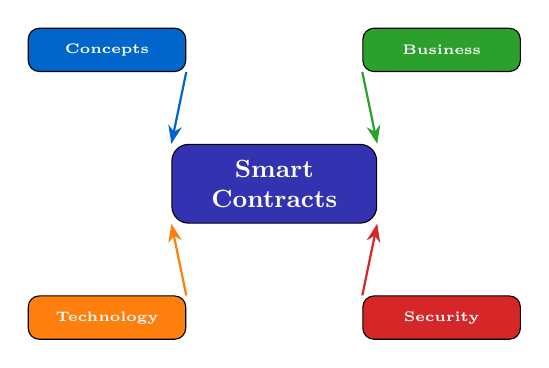
\begin{tikzpicture}[scale=0.85]
  % Central node
  \node[draw,fill=mlpurple,text=white,rounded corners=6pt,
        minimum width=2.6cm,minimum height=1.0cm,align=center,font=\small\bfseries]
        (sc) at (0,0) {Smart\\Contracts};
  % Surrounding concepts
  \node[draw,fill=mlblue,text=white,rounded corners=4pt,
        minimum width=2.0cm,minimum height=0.55cm,align=center,font=\tiny\bfseries]
        (c1) at (-2.5,2.0) {Concepts};
  \node[draw,fill=mlgreen,text=white,rounded corners=4pt,
        minimum width=2.0cm,minimum height=0.55cm,align=center,font=\tiny\bfseries]
        (c2) at (2.5,2.0) {Business};
  \node[draw,fill=mlorange,text=white,rounded corners=4pt,
        minimum width=2.0cm,minimum height=0.55cm,align=center,font=\tiny\bfseries]
        (c3) at (-2.5,-2.0) {Technology};
  \node[draw,fill=mlred,text=white,rounded corners=4pt,
        minimum width=2.0cm,minimum height=0.55cm,align=center,font=\tiny\bfseries]
        (c4) at (2.5,-2.0) {Security};
  \draw[-{Stealth},thick,mlblue] (c1.south east) -- (sc.north west);
  \draw[-{Stealth},thick,mlgreen] (c2.south west) -- (sc.north east);
  \draw[-{Stealth},thick,mlorange] (c3.north east) -- (sc.south west);
  \draw[-{Stealth},thick,mlred] (c4.north west) -- (sc.south east);
\end{tikzpicture}
\vspace{3mm}
\begin{exampleblock}{One Sentence Summary}
\footnotesize
Smart contracts transform \emph{trust in institutions} into \emph{trust in code}, enabling a new paradigm of programmable, transparent, and automated agreements.
\end{exampleblock}
\end{columns}
\bottomnote{This lecture provided a comprehensive introduction to smart contracts -- from concept and history through business applications to technical foundations and security}
\end{frame}

% Frame 54: Smart Contracts: From L14 to the Course
\begin{frame}{Smart Contracts: From L14 to the Course}
\centering
\vspace{2mm}
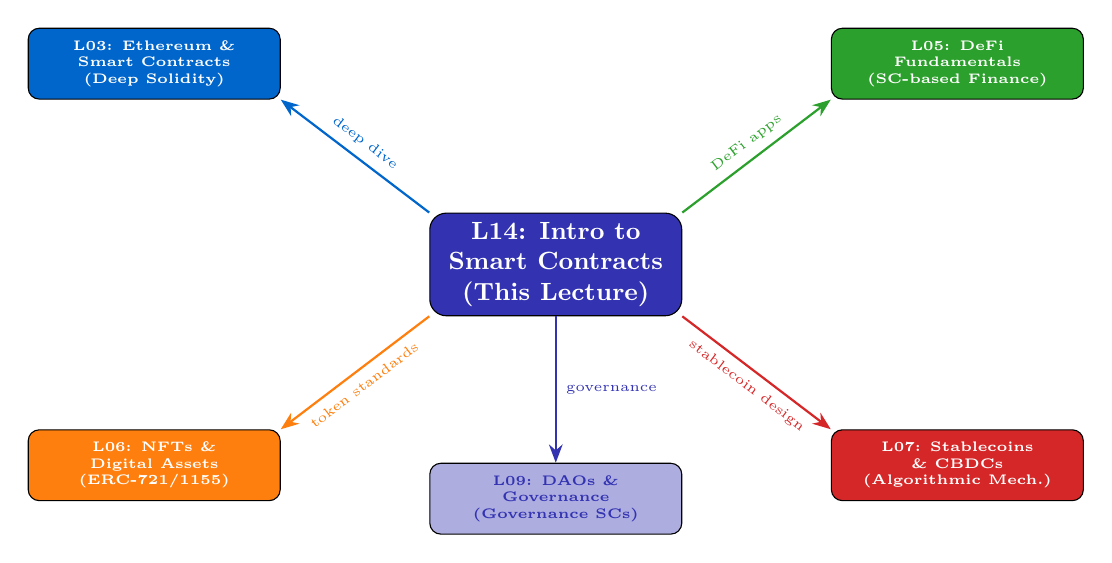
\begin{tikzpicture}[scale=0.85]
  % Central node: this lecture
  \node[draw,fill=mlpurple,text=white,rounded corners=6pt,
        minimum width=3.2cm,minimum height=1.2cm,align=center,font=\small\bfseries]
        (l14) at (6.0,0) {L14: Intro to\\Smart Contracts\\(This Lecture)};

  % Connected lectures
  \node[draw,fill=mlblue,text=white,rounded corners=4pt,
        minimum width=3.2cm,minimum height=0.9cm,align=center,font=\tiny\bfseries]
        (l03) at (0,3.0) {L03: Ethereum \&\\Smart Contracts\\(Deep Solidity)};
  \node[draw,fill=mlgreen,text=white,rounded corners=4pt,
        minimum width=3.2cm,minimum height=0.9cm,align=center,font=\tiny\bfseries]
        (l05) at (12.0,3.0) {L05: DeFi\\Fundamentals\\(SC-based Finance)};
  \node[draw,fill=mlorange,text=white,rounded corners=4pt,
        minimum width=3.2cm,minimum height=0.9cm,align=center,font=\tiny\bfseries]
        (l06) at (0,-3.0) {L06: NFTs \&\\Digital Assets\\(ERC-721/1155)};
  \node[draw,fill=mlred,text=white,rounded corners=4pt,
        minimum width=3.2cm,minimum height=0.9cm,align=center,font=\tiny\bfseries]
        (l07) at (12.0,-3.0) {L07: Stablecoins\\\& CBDCs\\(Algorithmic Mech.)};
  \node[draw,fill=mllavender,text=mlpurple,rounded corners=4pt,
        minimum width=3.2cm,minimum height=0.9cm,align=center,font=\tiny\bfseries]
        (l09) at (6.0,-3.5) {L09: DAOs \&\\Governance\\(Governance SCs)};

  % Arrows from L14 to connected lectures
  \draw[-{Stealth},thick,mlblue] (l14.north west) -- (l03.south east)
        node[midway,above,font=\tiny,text=mlblue,sloped] {deep dive};
  \draw[-{Stealth},thick,mlgreen] (l14.north east) -- (l05.south west)
        node[midway,above,font=\tiny,text=mlgreen,sloped] {DeFi apps};
  \draw[-{Stealth},thick,mlorange] (l14.south west) -- (l06.north east)
        node[midway,below,font=\tiny,text=mlorange,sloped] {token standards};
  \draw[-{Stealth},thick,mlred] (l14.south east) -- (l07.north west)
        node[midway,below,font=\tiny,text=mlred,sloped] {stablecoin design};
  \draw[-{Stealth},thick,mlpurple] (l14.south) -- (l09.north)
        node[midway,right,font=\tiny,text=mlpurple] {governance};
\end{tikzpicture}
\vspace{3mm}
\begin{columns}[T]
\column{0.5\textwidth}
\begin{block}{This Lecture Is Your Foundation}
\footnotesize
\begin{itemize}
  \item Concepts introduced here appear throughout the course
  \item L03 goes deep into Solidity programming
  \item L05--L07 explore DeFi, NFTs, and stablecoins in detail
\end{itemize}
\end{block}
\column{0.5\textwidth}
\begin{block}{Recommended Path}
\footnotesize
\begin{itemize}
  \item Start here (L14) for the big picture
  \item Then L03 for technical depth
  \item Then L05, L06, L07, L09 for applications
\end{itemize}
\end{block}
\end{columns}
\bottomnote{This standalone lecture is designed as an entry point -- every concept here is explored in greater depth in the corresponding specialized lectures}
\end{frame}

% Frame 55: Discussion Questions
\begin{frame}{Discussion Questions}
\begin{enumerate}
\item \textcolor{mlblue}{\textbf{Can ``code is law'' coexist with legal systems designed for human ambiguity?}}

\footnotesize If a smart contract executes as programmed but produces an outcome that a court would deem unfair, which system should prevail? How do we reconcile deterministic code with the nuance of human justice?

\normalsize
\vspace{3mm}
\item \textcolor{mlgreen}{\textbf{If a smart contract has a bug that benefits one party, is exploiting it theft or fair use?}}

\footnotesize The DAO hacker argued they were using the contract ``as written.'' Where is the line between a legitimate transaction and an exploit? Does intent matter when the code is the final arbiter?

\normalsize
\vspace{3mm}
\item \textcolor{mlorange}{\textbf{Which industry will be most transformed by smart contracts in the next decade?}}

\footnotesize Finance, supply chain, healthcare, real estate, and insurance are all candidates. What factors determine where automation and disintermediation create the most value?

\normalsize
\vspace{3mm}
\item \textcolor{mlpurple}{\textbf{How should smart contract auditing be regulated -- like financial auditing?}}

\footnotesize With billions at stake, should audit firms face liability for missed vulnerabilities? Should auditing standards be mandated by regulation, or is the market sufficient?
\end{enumerate}
\bottomnote{These questions have no simple answers -- they sit at the intersection of technology, law, ethics, and economics; discuss with your peers and form your own positions}
\end{frame}

% Frame 56: Further Reading and Resources
\begin{frame}{Further Reading and Resources}
\begin{columns}[T]
\column{0.5\textwidth}
\begin{block}{\textcolor{mlblue}{Books}}
\footnotesize
\begin{itemize}
  \item \textbf{Mastering Ethereum} -- Antonopoulos \& Wood (comprehensive technical reference)
  \item \textbf{Solidity Programming Essentials} -- Modi (practical introduction)
  \item \textbf{The Infinite Machine} -- Russo (Ethereum history, non-technical)
  \item \textbf{How to DeFi: Beginner} -- CoinGecko (accessible DeFi overview)
\end{itemize}
\end{block}
\vspace{2mm}
\begin{block}{\textcolor{mlgreen}{Websites and Documentation}}
\footnotesize
\begin{itemize}
  \item \textbf{ethereum.org} -- official Ethereum documentation and tutorials
  \item \textbf{solidity-by-example.org} -- learn Solidity through annotated examples
  \item \textbf{etherscan.io} -- explore contracts, transactions, and tokens on-chain
  \item \textbf{defillama.com} -- DeFi analytics and protocol rankings
\end{itemize}
\end{block}

\column{0.5\textwidth}
\begin{block}{\textcolor{mlorange}{Development Tools}}
\footnotesize
\begin{itemize}
  \item \textbf{Remix IDE} -- browser-based Solidity editor and debugger
  \item \textbf{Hardhat} -- professional Ethereum development framework (JavaScript)
  \item \textbf{Foundry} -- fast, Rust-based testing and deployment toolkit
  \item \textbf{OpenZeppelin} -- audited, reusable smart contract libraries
\end{itemize}
\end{block}
\vspace{2mm}
\begin{block}{\textcolor{mlpurple}{Academic Resources}}
\footnotesize
\begin{itemize}
  \item IEEE and ACM papers on smart contract \textbf{formal verification}
  \item \textbf{Atzei et al.} (2017): ``A Survey of Attacks on Ethereum Smart Contracts''
  \item \textbf{Buterin} (2014): Ethereum Whitepaper
  \item \textbf{Szabo} (1997): ``Formalizing and Securing Relationships on Public Networks''
\end{itemize}
\end{block}
\end{columns}
\bottomnote{Smart contract development is a rapidly evolving field -- stay current with the latest tools, standards, and security practices through continuous learning}
\end{frame}

\end{document}
